\chapter{\texorpdfstring{\textsc{Hanna}}{Hanna}: A Corpus of Human-ANnotated NArratives for {\asg} Evaluation}
\citationChap{
    This is a story of the past. The story of him and her, only fifteen days long, concerning a certain grail.
    }{\textit{Fate/stay night: Last Episode}}
\label{chap:hanna}
\minitoc
\newpage

\chapabstract{
    In order to use our human evaluation criteria (\autoref{sec:human_criteria}) and to conduct a meta-evaluation with our proposed framework (\autoref{sec:meta_evaluation_framework}), we need an appropriate dataset of stories. In this chapter, we describe the building process of {\hanna}, our corpus of Human ANnotated NArratives. We begin by reviewing  corpora related to {\asgfull} and find that no existing dataset contains human annotations {\wrt}\ specific criteria of story quality (\autoref{sub:asg_corpora}). We then review and select {\asg} systems (\autoref{sub:neural_asg}) in order to build our own corpus, \hanna, specifically designed for {\asg} evaluation. The first version of {\hanna} contains 1,056 stories produced by 11 systems and aligned on 96 prompts (\autoref{sub:hanna_v1}). We perform an annotation experiment on {\hanna} V1, asking human raters to grade each story {\wrt} our six human criteria. We analyze the overall and system-level correlations between our human criteria, and confirm that they allow for a standardized and extensive human evaluation (\autoref{sub:evaluating_human_criteria}). We also observe that large pre-trained language models, namely {\gptt}, produce the best results for ASG (\autoref{sub:comparing_asg_systems}). Finally, we use {\llmfull}s to augment {\hanna} with 480 new stories (\autoref{sub:llm_methodology_asg}) and 150k+ annotations (\autoref{sub:llm_methodology_ase}), and observe that {\llm}s are rated more highly than humans when evaluated by two different {\llm}s (\autoref{sub:asg1_analysis}).
}

\section{Introduction}

Performing evaluation experiments in {\nlp} requires appropriate resources and, especially, a fitting dataset. {\nlp} research in particular has a long history of developing corpora and benchmarks to support the development and evaluation of algorithms for multiple tasks.

Many early initiatives focused on large-scale annotation collection to assist data-driven methods for low-level tasks like part-of-speech tagging \citep{marcus1993building} and named entity recognition \citep{grishman1996message}. Other early benchmarks were primarily intended to explore the information found in linguistic knowledge and context, such as the Message Understanding Conference (MUC) benchmarks for information extraction \citep{sundheim1993tipster} and the Automatic Content Extraction (ACE) benchmarks for relation extraction and coreference resolution \citep{doddington2004automatic}. Other benchmarks were centered on reading comprehension \citep{hirschman1999deep} and question answering \citep{kocisky2018narrativeqa}. 

The scope of these benchmarks has ranged from more general tasks such as textual entailment \citep{dagan2006pascal} to very specialized tasks like reference resolution \citep{levesque2011winograd}. Some benchmarks, like GLUE \citep{wang-etal-2018-glue}, are made up of multiple tasks, whereas others concentrate primarily on one task only: for instance, the \textsc{SQuAD} benchmark \citep{rajpurkar2016squad} contains more than 100,000 questions for machine comprehension.

In this chapter, we elaborate on the building process of {\hanna}, our corpus of Human ANnotated NArratives designed for the evaluation of {\asgfull}.

\section{Design Decisions for Building \hanna}
\label{sec:decision_process_hanna}

We begin by surveying existing corpora of written stories (\autoref{sub:asg_corpora}) to examine whether how appropriate they are for our benchmarking goals; in particular, we look for corpora with extensive human annotations {\wrt}\ specific evaluation criteria.

\subsection{Survey of Corpora Related to Automatic Story Generation}
\label{sub:asg_corpora}

\paragraph{\roc.}
The first major, easily accessible dataset of stories found in the recent literature is {\roc} \citep{mostafazadeh2016corpus}, a crowdsourced corpus of 50k 5-sentence stories with titles. {\roc} was designed for the Story Cloze Test, an evaluation framework for story understanding that consists in predicting the final sentence of a story given the four previous sentences. {\roc} includes diverse causal and temporal relationships across a broad spectrum of situations, and its multiple nonfictional short stories constitute effective training data for building story generation models. Examples of stories from {\roc} can be found in \autoref{tab:rocstories}. As part of the Story Cloze Test evaluation framework they introduce, every story has an alternative ``wrong'' ending that complements the canonical ``right'' ending (see \autoref{tab:story_cloze_test}).

\begin{table}[h!]
\small
\centering
\begin{tabular}{lp{0.7\columnwidth}}
\toprule
    \textbf{Title} & \textbf{Five-sentence Story} \\
\midrule
    The Test & Jennifer has a big exam tomorrow. She got so stressed, she pulled an all-nighter. She went into class the next day, weary as can be. Her teacher stated that the test is postponed for next week. Jennifer felt bittersweet about it. \\
\midrule
    The Hurricane & Morgan and her family lived in Florida. They heard a hurricane was coming. They decided to evacuate to a relative's house. They arrived and learned from the news that it was a terrible storm. They felt lucky they had evacuated when they did. \\
\midrule
    Spaghetti Sauce & Tina made spaghetti for her boyfriend. It took a lot of work, but she was very proud. Her boyfriend ate the whole plate and said it was good. Tina tried it herself, and realized it was disgusting. She was touched that he pretended it was good to spare her feelings. \\
\bottomrule
\end{tabular}
\caption{Example stories from \roc\ \citep{mostafazadeh2016corpus}.}
\label{tab:rocstories}
\end{table}

\begin{table}[h!]
\small
\centering
\begin{tabular}{p{0.45\columnwidth}p{0.22\columnwidth}p{0.22\columnwidth}}
\toprule
    \textbf{Context} & \textbf{Right Ending} & \textbf{Wrong Ending} \\
\midrule
    Karen was assigned a roommate her first year of college. Her roommate asked her to go to a nearby city for a concert. Karen agreed happily. The show was absolutely exhilarating. & Karen became good friends with her roommate. & Karen hated her roommate. \\
\midrule
    Jim got his first credit card in college. He didn’t have a job so he bought everything on his card. After he graduated he amounted a \$10,000 debt. Jim realized that he was foolish to spend so much money. & Jim decided to devise a plan for repayment. & Jim decided to open another credit card. \\
\midrule
    Gina misplaced her phone at her grandparents. It wasn’t anywhere in the living room. She realized she was in the car before. She grabbed her dad’s keys and ran outside. & She found her phone in the car. & She didn’t want her phone anymore. \\
\bottomrule
\end{tabular}
\caption{Example stories from the Story Cloze Test \citep{mostafazadeh2016corpus}.}
\label{tab:story_cloze_test}
\end{table}

\begin{table}[h!]
\small
\centering
\begin{tabular}{lp{0.15\columnwidth}p{0.15\columnwidth}p{0.15\columnwidth}p{0.15\columnwidth}p{0.15\columnwidth}}
\toprule
    & \textbf{1} & \textbf{2} & \textbf{3} & \textbf{4} & \textbf{5} \\
\midrule
& 
\includegraphics[width=\linewidth]{pictures/sind1.jpg} & 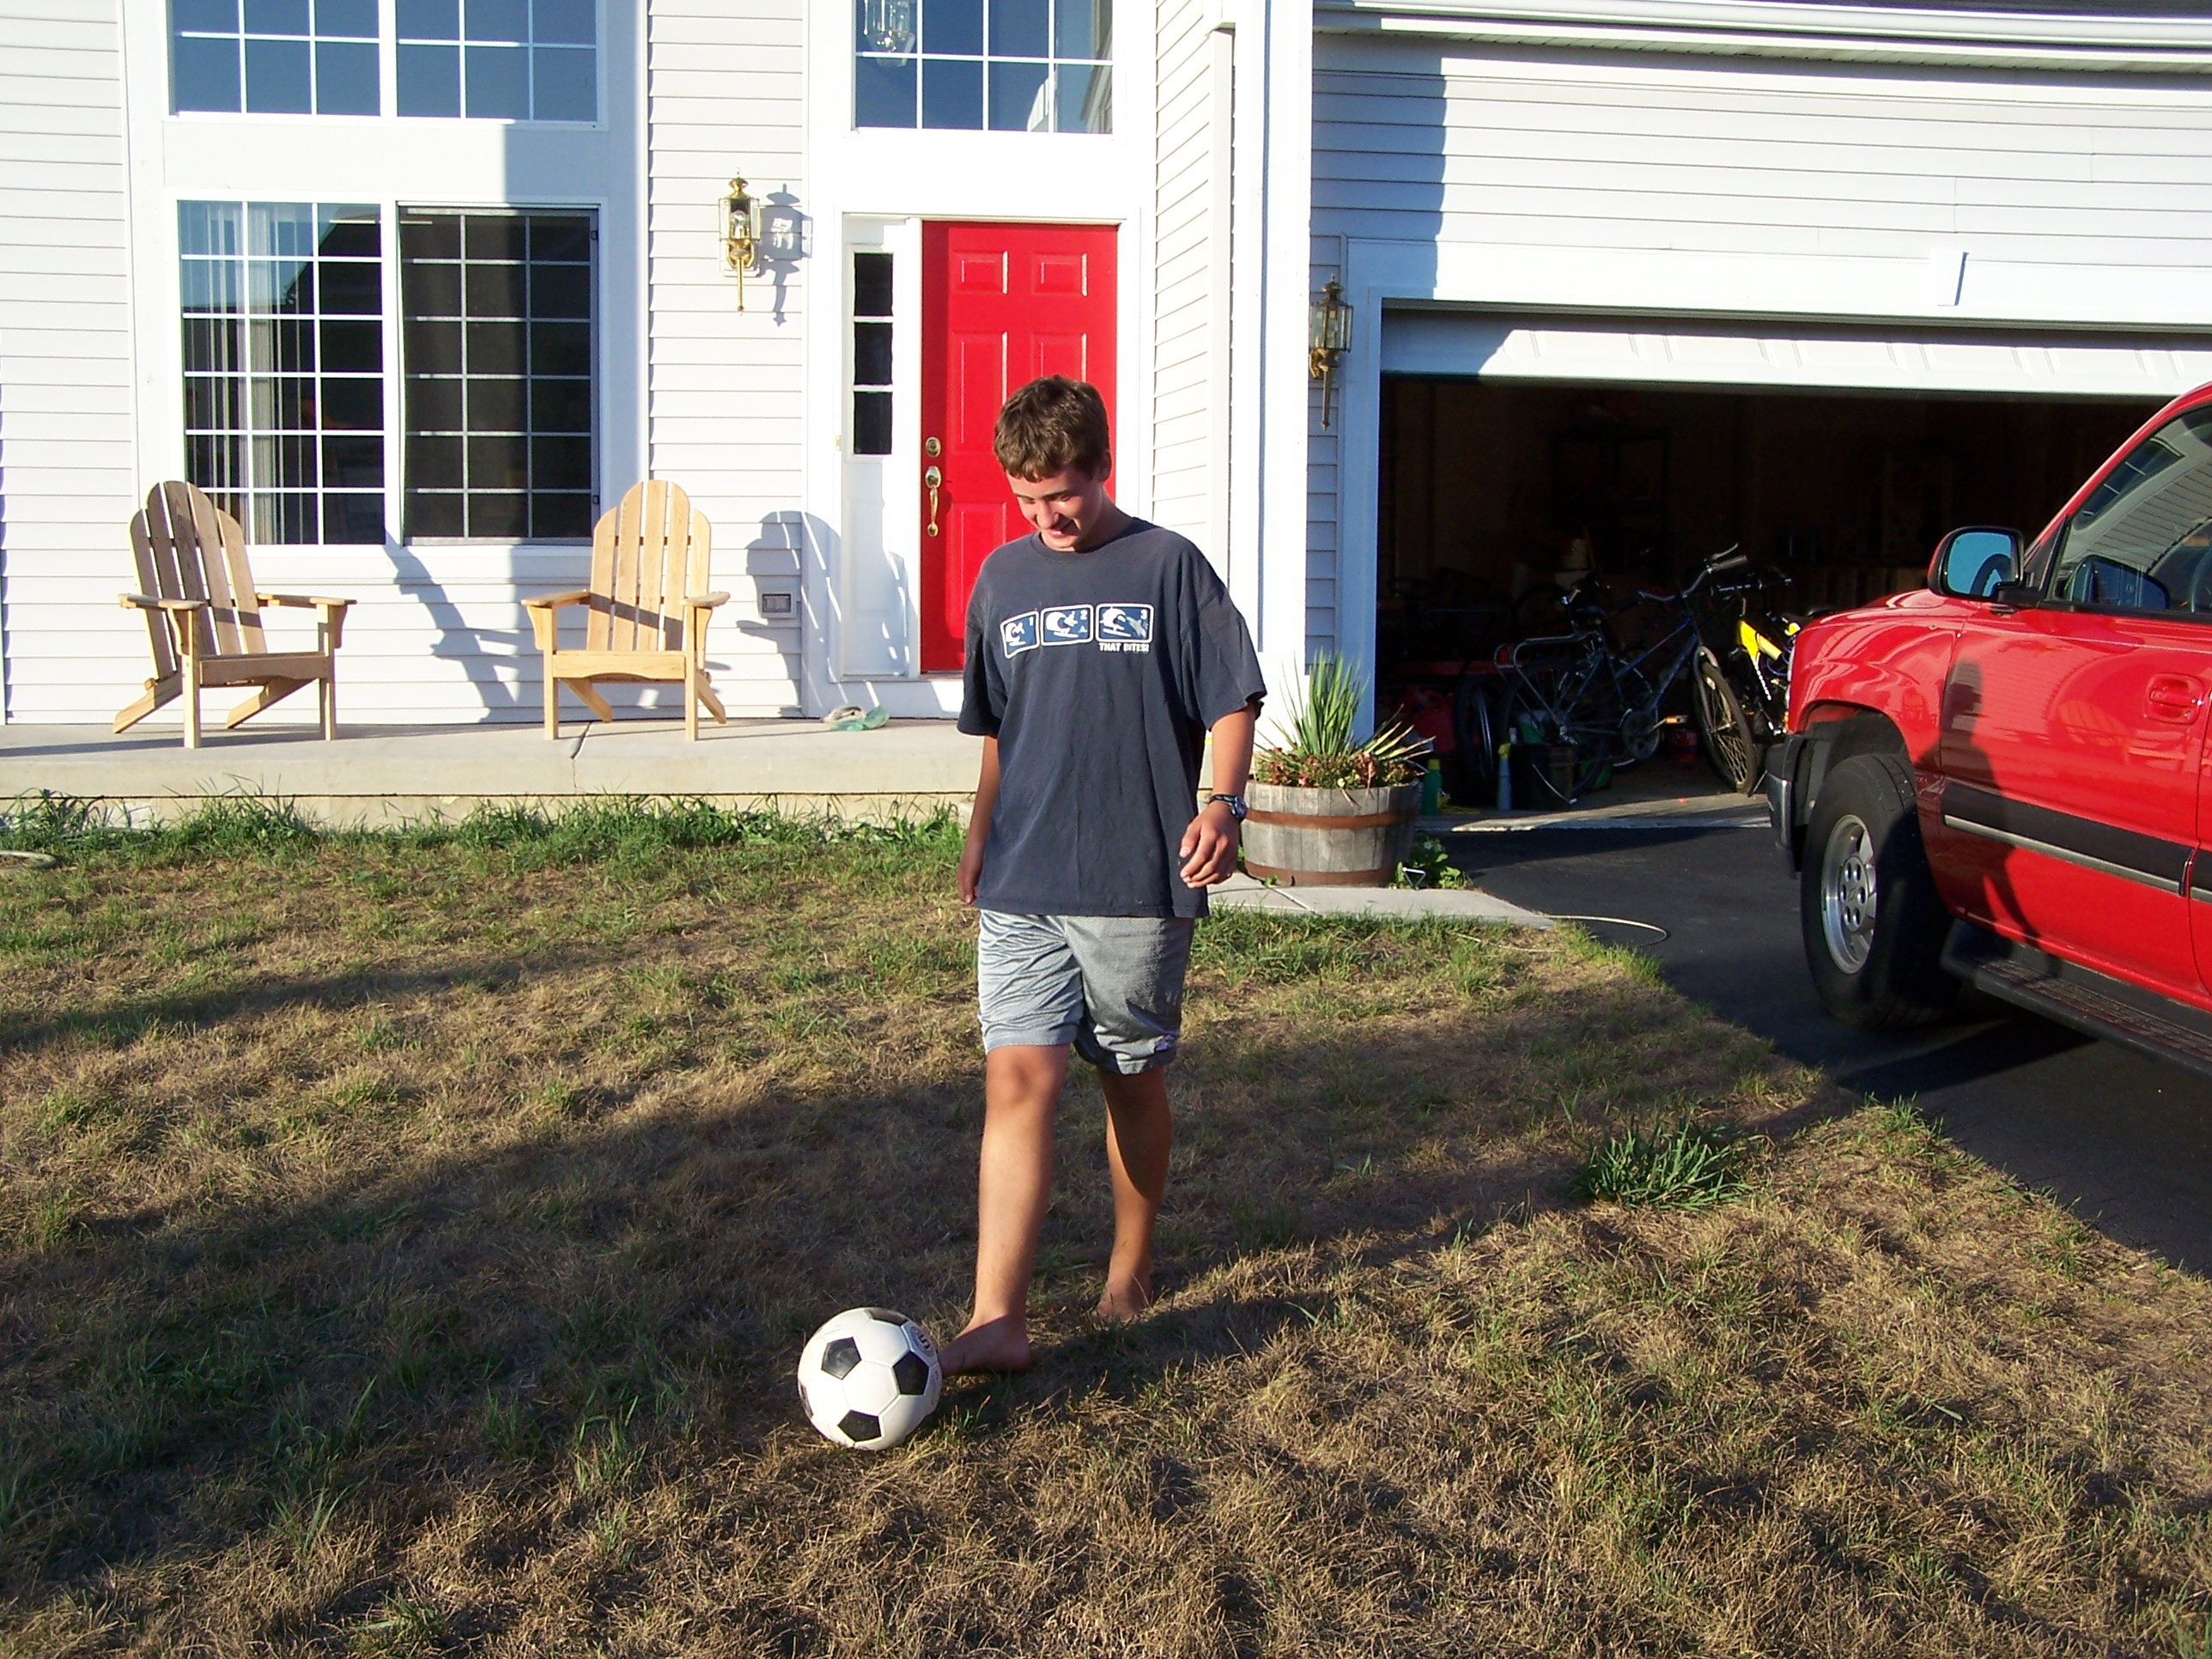
\includegraphics[width=\linewidth]{pictures/sind2.jpg} & 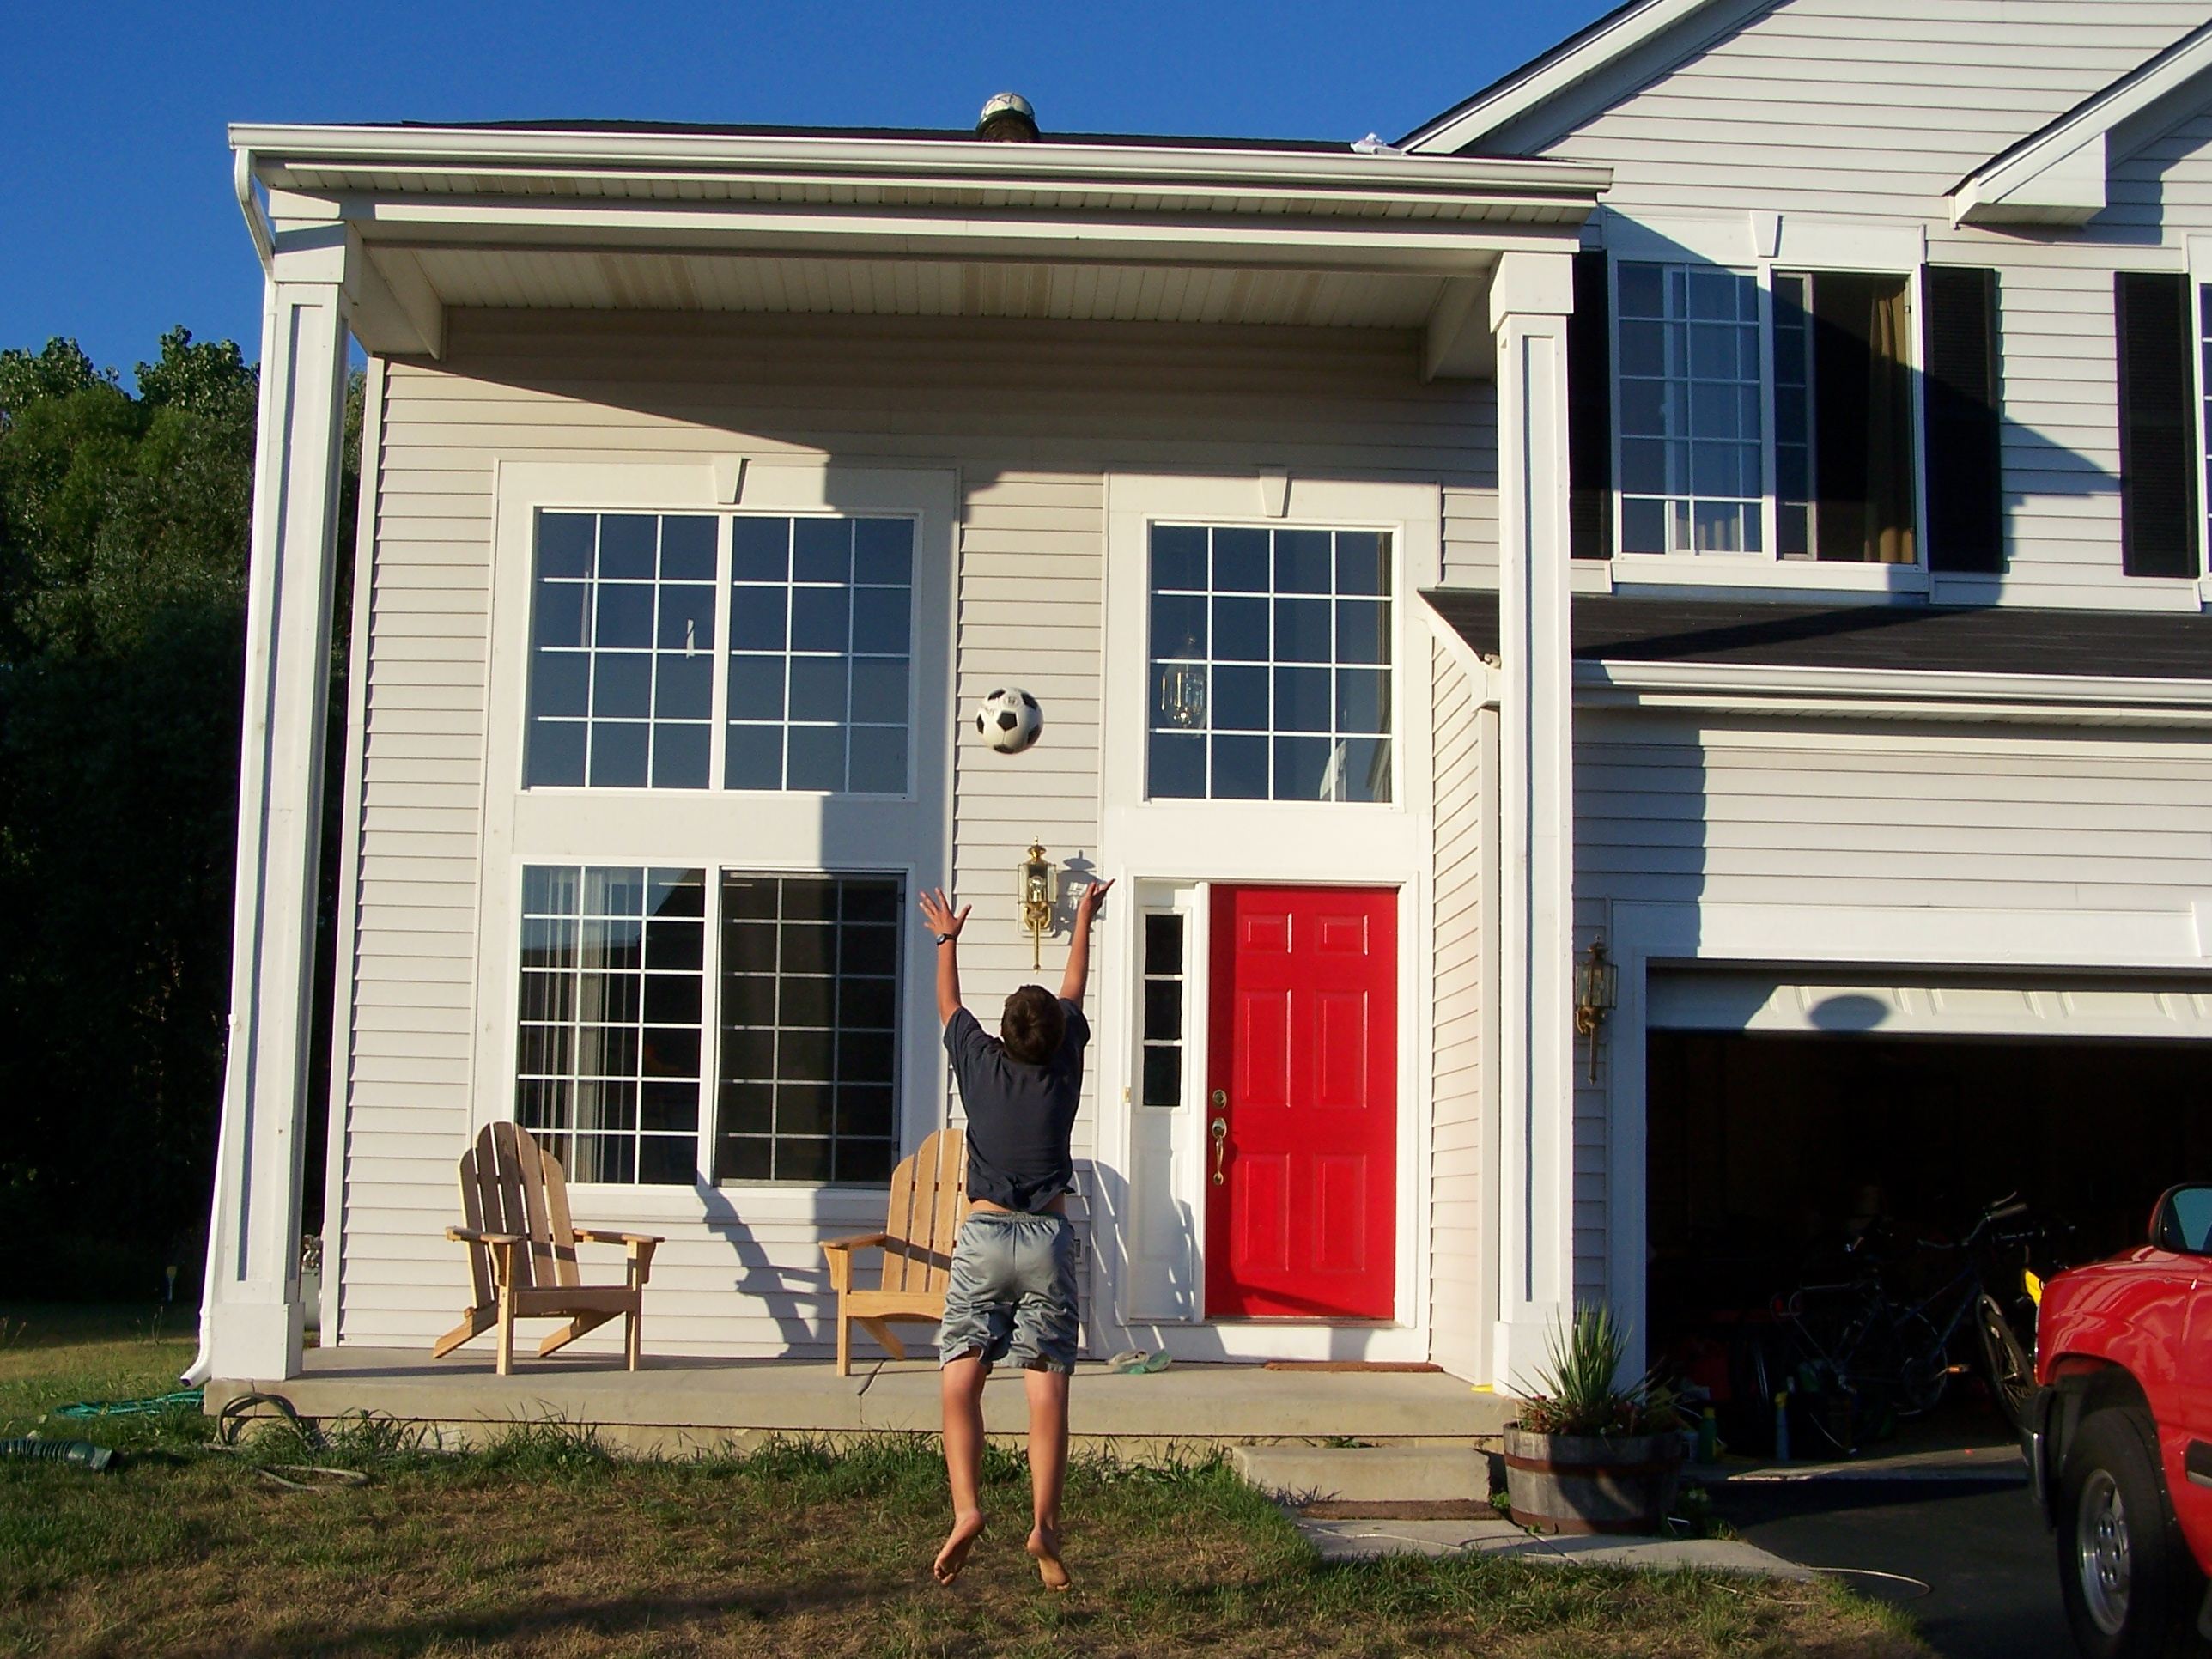
\includegraphics[width=\linewidth]{pictures/sind3.jpg} & 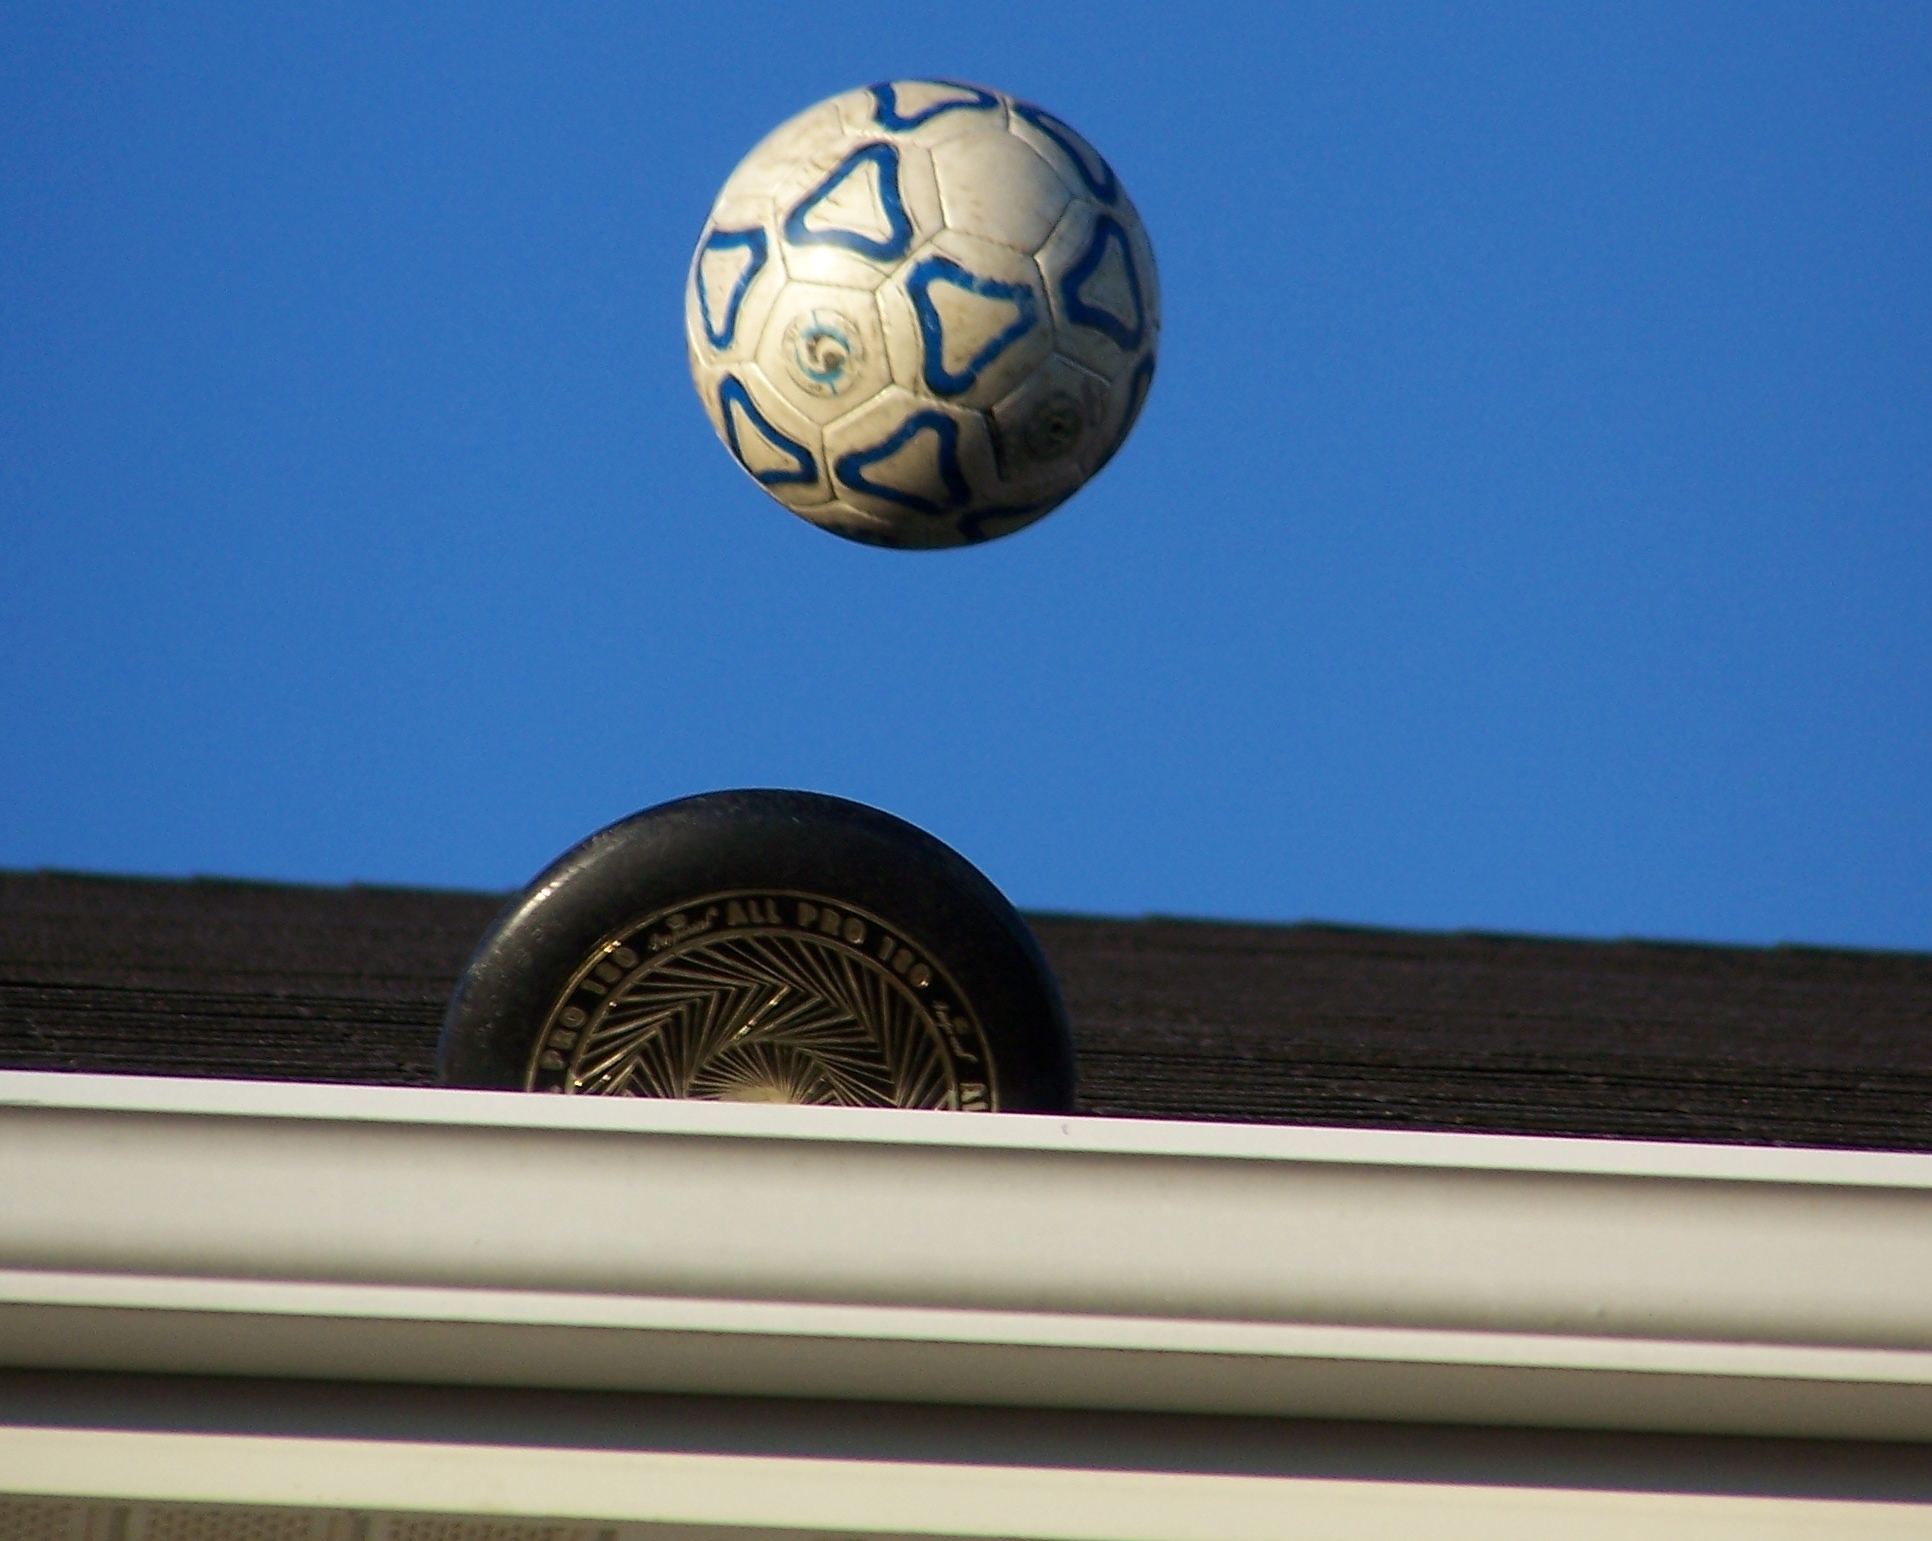
\includegraphics[width=\linewidth]{pictures/sind4.jpg} & 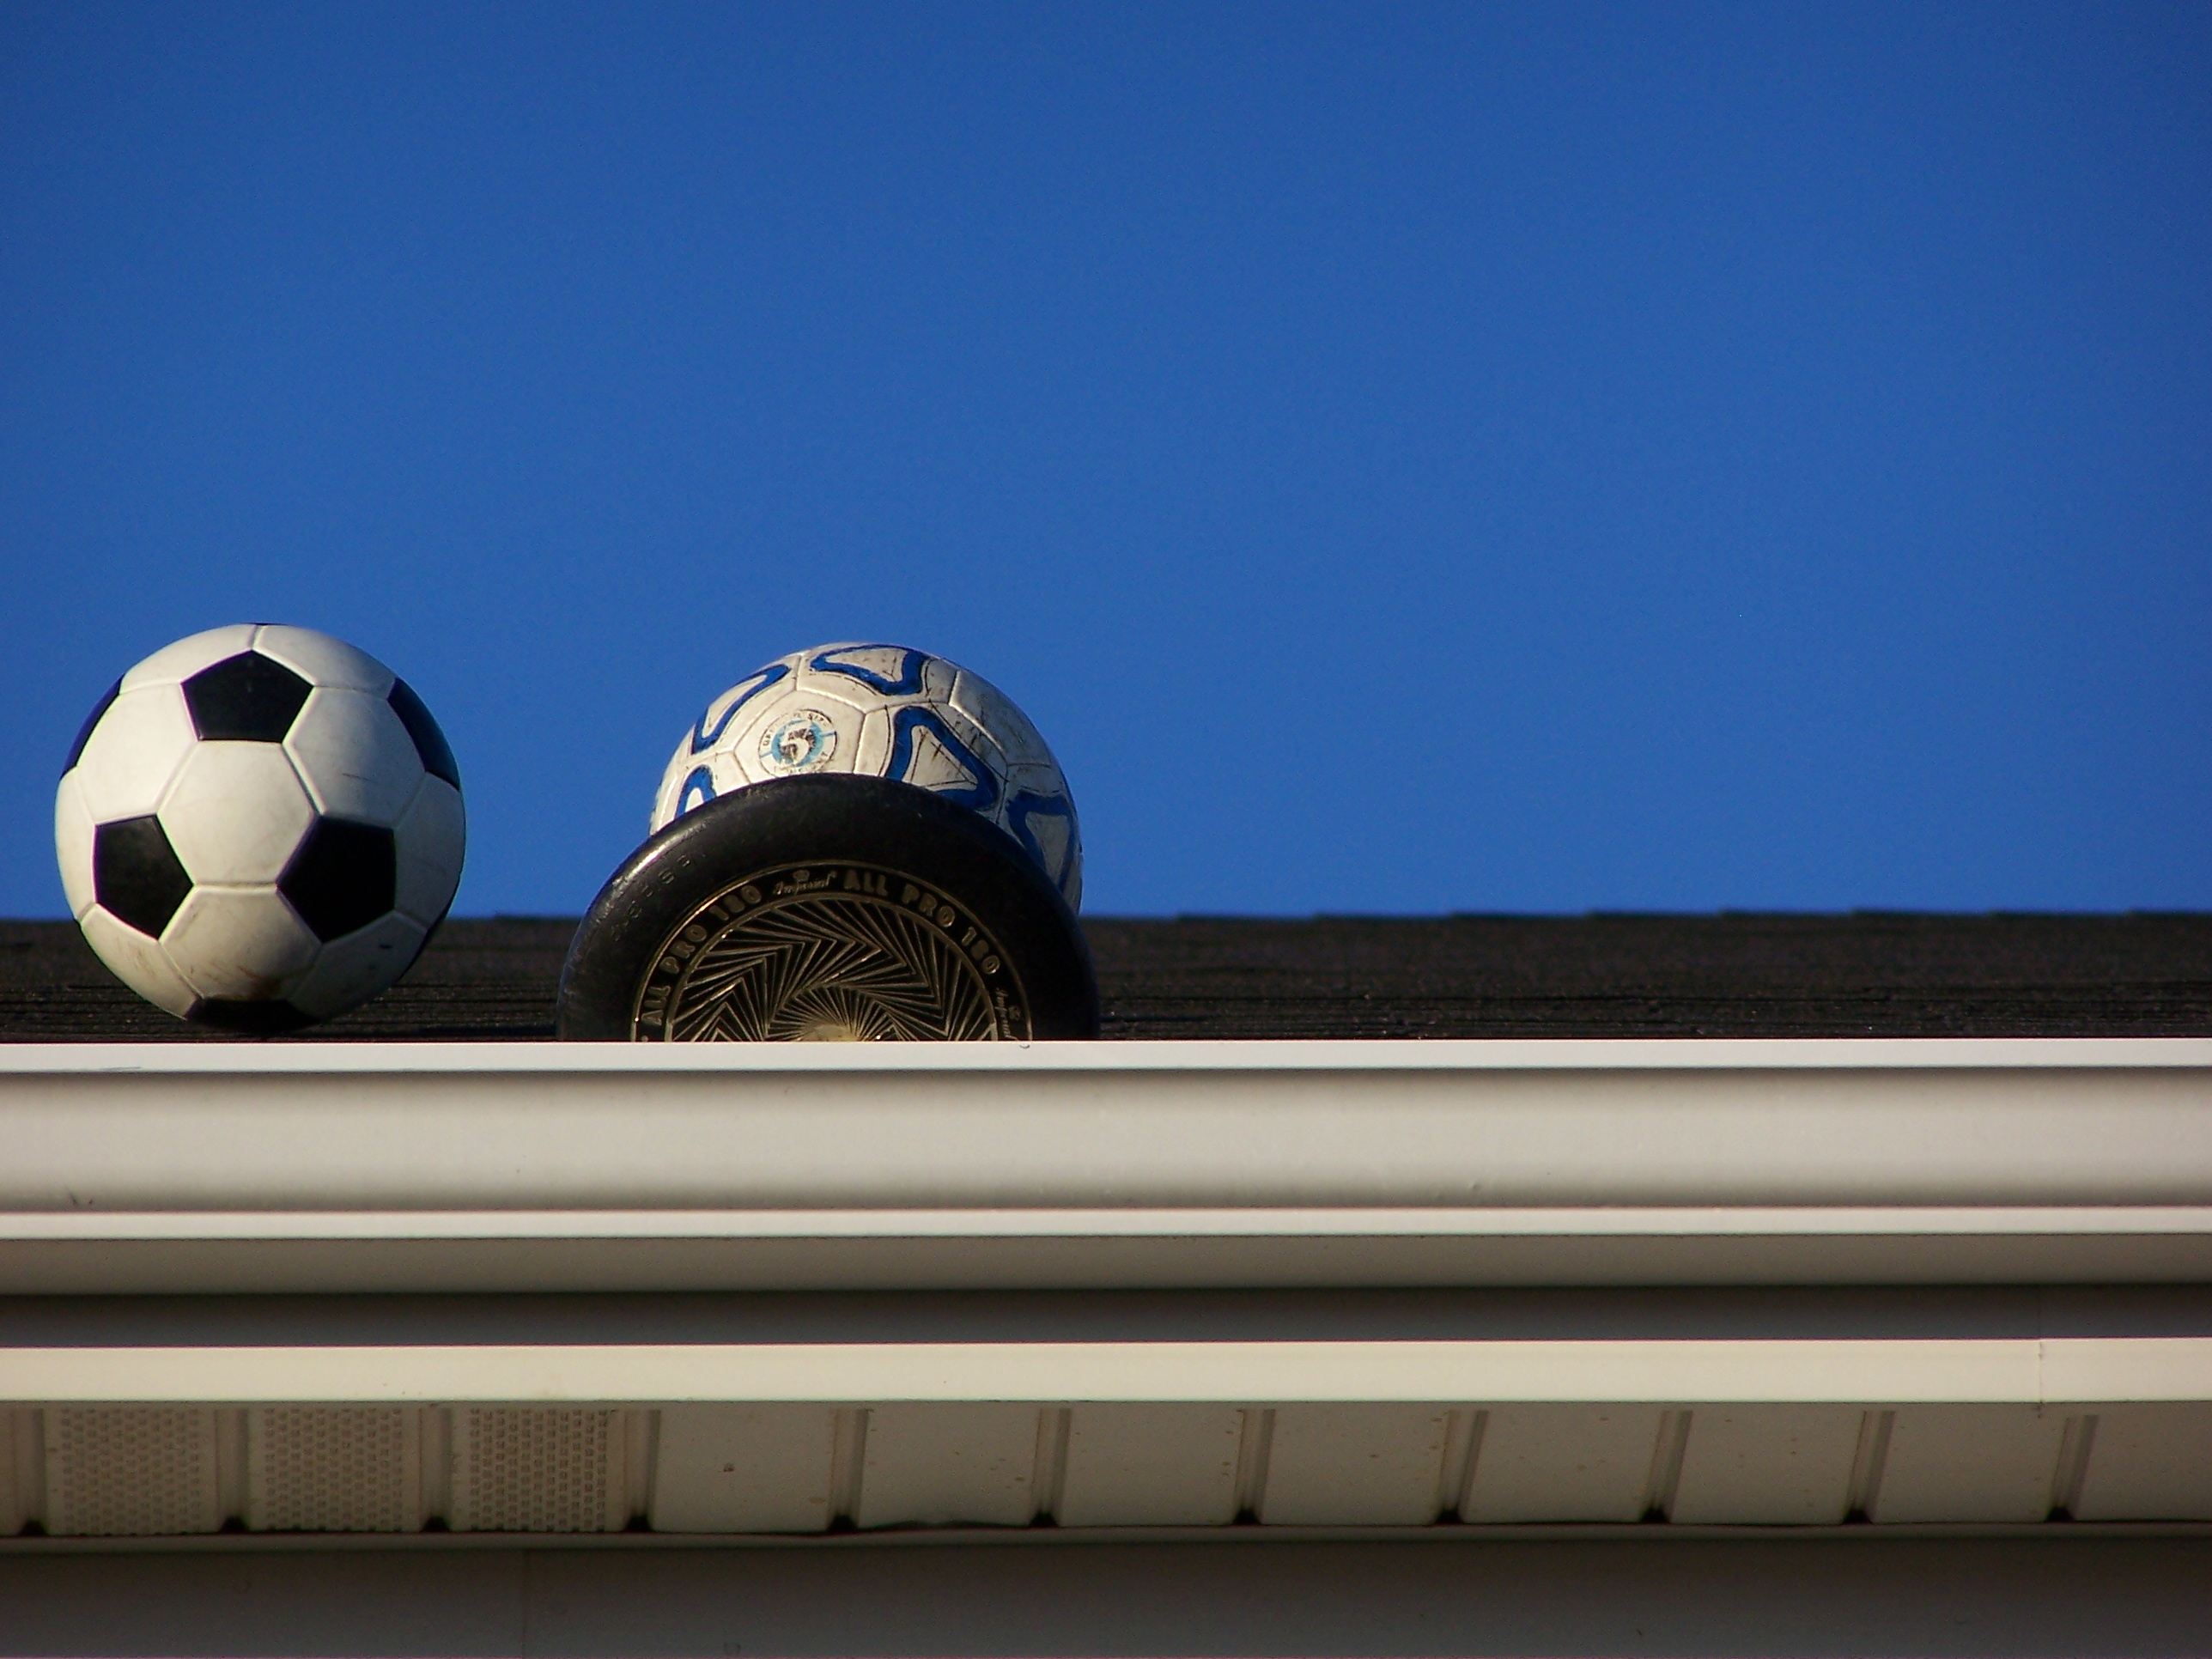
\includegraphics[width=\linewidth]{pictures/sind5.jpg} \\
\midrule
DII & A black frisbee is sitting on top of a roof. & A man playing soccer outside of a white house with a red door. & The boy is throwing a soccer ball by the red door. & A soccer ball is over a roof by a frisbee in a rain gutter. & Two balls and a frisbee are on top of a roof. \\
\midrule
DIS	& A roof top with a black frisbee laying on the top of the edge of it. & A man is standing in the grass in front of the house kicking a soccer ball. & A man is in the front of the house throwing a soccer ball up. & A blue and white soccer ball and black Frisbee are on the edge of the roof top. & Two soccer balls and a Frisbee are sitting on top of the roof top. \\
\midrule
SIS	& A discus got stuck up on the roof. & Why not try getting it down with a soccer ball? & Up the soccer ball goes. & It didn't work so we tried a volley ball. & Now the discus, soccer ball, and volleyball are all stuck on the roof. \\
\bottomrule
\end{tabular}
\caption{Example story from \sind\ \citep{huang2016visual}.}
\label{tab:sind}
\end{table}

\paragraph{\sind.}
\citet{huang2016visual} developed \sind\ (Sequential Images Narratives Dataset), the first dataset for sequential vision-to-language, for the task of visual storytelling. \sind\ contains 81,743 unique photos in 20,211 sequences, with accompanying captions and stories. The data is organized in three categories of language, so as to assess the importance of temporal context and narrative language: (1) Descriptions of images-in-isolation (\textsc{DII}), (2) Descriptions of images-in-sequence (\textsc{DIS}) and (3) Stories for images-in-sequence (\textsc{SIS}). They train {\rnn}-based story generation models on {\sind} and, using simple heuristics, perform experiments that demonstrate that story generation is fundamentally different from caption generation. Examples are shown on \autoref{tab:sind}.

\begin{table}[h!]
\small
\centering
\begin{tabular}{p{0.3\columnwidth}p{0.6\columnwidth}}
\toprule
    \textbf{Prompt} & \textbf{Story} \\
\midrule
    You've finally managed to discover the secret to immortality. Suddenly, Death appears before you, hands you a business card, and says, ``When you realize living forever sucks, call this number, I've got a job offer for you .'' & So many times have I walked on ruins, the remainings of places that I loved and got used to.. At first I was scared, each time I could feel my city, my current generation collapse, break into the black hole that thrives within it, I could feel humanity, the way I'm able to feel my body.. After a few hundred years, the pattern became obvious, no longer the war and damage that would devastate me over and over again in the far past was effecting me so dominantly. [...] \\
\midrule
    The moon is actually a giant egg, and it has just started to hatch. & - Week 18 aboard the Depth Reaver, Circa 2023 - I walk about the dull gray halls, the artificial gravity making my steps feel almost as if they were on land. Almost. I glance out a window as I pass it by. There's the sun, and there's the moon right there. And, of course, there's the Earth. I kinda miss it. Then again, space is pretty cool. It's got some brilliant views, and the wifi is surprisingly good. [...] \\
\midrule
    Write a horror story from the perspective of the antagonist. Make them as sympathetic as possible. & I don't want to cut off his head, but I don't really have a choice. I close my eyes and just wait for it to be over. My insides turn as I feel the swing connect. \textit{Quit being so weak! You've done this before.} The jock's girlfriend screams on cue, looks like she is going to faint. She has blonde hair and a blue dress patterned with diamonds. I see how scared she is, and I feel ashamed. I'm not the bad guy. [...] \\
\bottomrule
\end{tabular}
\caption{Example stories from \wpfan\ \citep{fan2018hierarchical}.}
\label{tab:writingprompts}
\end{table}

\paragraph{\wpfan.}
\citet{fan2018hierarchical} released the \wpfan\ dataset, which contains 300k human-written stories paired with writing prompts from Reddit's /r/WritingPrompts forum, where members encourage one another to write stories by providing story premises called prompts. Those prompts exhibit a wide range of themes and can be answered by multiple users. To be included in the dataset, stories had to be longer than 30 words, avoid inappropriate content, and be related to the prompt. They also introduce a hierarchical model with self-attention for story generation, and demonstrate that it produces stories which are more fluent and more relevant to the prompt than previous state-of-the-art models. Examples are shown on \autoref{tab:writingprompts}.

\paragraph{\rpguild.}
\citet{louis2018deep} collect a corpus of \rpg\ threads from the \href{https://roleplayerguild.com}{\texttt{roleplayerguild.com}} website. {\rpg}s are usually played in-person, but users can also play them online. Threads come in pairs: the first thread contains the description of the players' characters, with multiple attributes, and the second thread contains the actual game play where each player describes the actions they take when their turn comes. The \rpguild\ corpus is a collection of 1,544 {\rpg}s of different themes, such as adventure, romance and horror. An example is shown on \autoref{tab:rpguild}.

\begin{table}[h!]
\small
\centering
\begin{tabular}{p{0.45\columnwidth}p{0.45\columnwidth}}
\toprule
    \textbf{Character Description} & \textbf{Action Description} \\
\midrule
    Name: Ana Blackclaw; Age: 27; Gender: Female Appearance: Standing at a mighty 6’5, she is a giant among her fellow humans. Her face is light, though paler than the average man or woman’s, and is marked by scars. ... Her body is muscular, as it would have to be to carry both her armor and the hammer. Her light grey eyes nearly always keep a bored expression. Her canines seem a tad larger than the normal person’s. Preferred Weapon: Hammer. Preferred Armor: Heavy. Gift: Binoculars. Darksign: No. & She stopped dead in her tracks as the hissing began. A grumble escaped her as it did so, and she looked over to make sure the other woman was doing fine. Seeing that all was not entirely well, she allowed herself to slide down, her hand gripping the slope side once more to slow herself. Once that was accomplished, she reached out and grabbed the back of the girl’s neck, pulling her back to steady herself. The giant remained silent as she did so, and then glanced over to the nearby skeletons. They would be upon them soon. Her grip tightened on the hammer as she glanced from side to side. It would not be a fun fight. \\
\bottomrule
\end{tabular}
\caption{Example descriptions from \rpguild\ \citep{louis2018deep}.}
\label{tab:rpguild}
\end{table}

\paragraph{\pgnt.}
\citet{rae2019compressive} propose the \pgnt\ dataset, a new open-vocabulary language modelling benchmark derived from Project Gutenberg books that were published before 1919. The {\pgnt} dataset contains 28,752 books, which they use for evaluating their Compressive Transformer model against other state-of-the-art models. They find that training on {\pgnt} helps their model produce long-range stories with different writing styles.

\paragraph{\storium.}
\citet{akoury2020storium} release a dataset of 6k lengthy stories (125M tokens) collected from the {\storium} collaborative storytelling community. Each story comes with multiple human annotations describing the characters' background and attributes. Whereas \storium\ contains fewer stories than other datasets such as \roc\ and \wpfan, its stories are overall longer and contain on average 14 narrator prompts per story and 41 annotations. They integrate language models onto {\storium} to enable users to generate and edit story continuations. They compute automatic evaluation measures scores over those edits and find that they correlate well with human ratings and feedback from user studies. 

\paragraph{\openmeva.}
\citet{guan2021openmeva} propose \openmeva, a benchmark for evaluating open-ended story generation metrics. OpenMEVA can be used to perform multiple tests on evaluation measures: (a) correlation with human judgments; (b) generalization to various model outputs and datasets; (c) story coherence judgment; and (d) robustness to perturbations. {\openmeva} comes with both automatically-generated test cases and manually-annotated stories. They evaluate current measures on {\openmeva} and find that they fail to recognize incoherence at the discourse-level correlate poorly with human judgments.

\begin{table}
    \centering
    \begin{tabular}{llcr}
        \toprule
        \textbf{Name} & \textbf{Type} & \textbf{Annotations} & \textbf{\# Words} \\
        \midrule
        \roc & Title + Story & \xmark & 80 \\
        \sind & Pictures + Story & \xmark & 80 \\
        \wpfan & Prompt + Story & \xmark & 750 \\
        \rpguild & RPG Thread & \xmark & 3,000 \\
        \pgnt & Book & \xmark & 69,000 \\
        \storium & Collaborative Story & \pmark & 19,000 \\
        \openmeva & Title/Prompt + Story & \pmark & 400 \\
        \bottomrule
    \end{tabular}
    \caption{Overview of existing story generation corpora. No corpus provides annotations on different criteria of story quality.}
    \label{tab:overview_corpora}
\end{table}

\subsubsection{Takeaways}
An overview of the reviewed corpora can be found in \autoref{tab:overview_corpora}. Most notably, none of the datasets we reviewed provided annotations {\wrt}\ specific evaluation criteria for story quality. {\storium} contains annotations that indicated whether story components were relevant to one another, while the {\openmeva} dataset \citep{guan2021openmeva} contained human annotations on a single criterion, ``overall quality'', which is negatively defined {\wrt}\ several error types. We therefore set out to create our own dataset for {\asg} evaluation. To that end, we need to select story generation models: we review the existing {\asg} systems in the next section.

\subsection{State-of-the-Art Models for Automatic Story Generation}
\label{sub:neural_asg}

The Automatic Story Generation task has been tackled with a variety of approaches, as shown in \autoref{sec:preneural_asg}. However, neural network-based models now constitute the vast majority of \asg\ models: we review a number of those below. We can make a distinction between older RNN-based approaches and newer transformer-based approaches.

\subsubsection{RNN-based {\asg} Systems}

\paragraph{\tingle.}
One of the first neural network-based \asg\ models is \tingle, introduced by \citet{khalifa2017deeptingle}. {\tingle} is made of two main components: (1) the neural network that learns to generate words in the style of the training corpus and (2) a set of co-creativity tools which help refine the writing style. {\tingle}'s training data contains all the books by Chuck Tingle released until November 2016, for a total of 109 short stories and 2 novels, all with similar structure. \tingle 's neural network is a 6-layer architecture based on {\lstm}s and \glove\ embeddings. Through a user study, they show that \tingle\ is better than a Markov model at generating coherent and fluent text.

\paragraph{\etoe\ and \etos.}
\citet{martin2018event} present a technique for translating textual story data into event sequences. They decompose the task of {\asg} into the generation of successive, generalized events (\etoe) and the generation of natural language sentences from events (\etos). Both \etoe\ and \etos\ networks are recurrent multi-layer {\rnn} encoder-decoder networks. First, a human-written sentence is translated as one or more events, and the \etoe\ network generates successive events. The \etos\ network then translates the events back into natural language. They show that generalized events with full-length generalized sentences yields an increase \bleu\ scores.

\paragraph{\engen.}
\citet{clark-etal-2018-neural} propose an entity-based generation model which uses three sources of contextual information: the current sentence, the previous sentence, and the current state of all mentioned entities. \engen\ combines \stsa, an \lstm-based entity-unaware model with an attention mechanism, with \entnlm\ \citep{ji2017dynamic}, a language model that adds explicit tracking of entities. They show that the combination of the three contexts improves model performance on three tasks: mention generation, sentence selection, and sentence generation.

\paragraph{Controllable Story Generation.}
\citet{peng-etal-2018-towards} propose a general framework for interactive story generation focused on the extraction of two control factors, ending valence and storyline, and two generation tasks. An ending valence is a label that describes a happy, sad, or unknown ending, while a storyline is a sequence of words that summarizes the story. Both control factors are extracted from the {\roc} dataset. The task of ending-valence controlled generation consists in the generation of a story ending given the first four senteces of a story and an ending valence. They use an {\lstm}-based conditional language model for it. For storyline-controlled generation, the goal is to generate a five-sentence story from a storyline. Here, they use a \seqseq\ model with attention. Through automatic and human evaluation, they show that their models generate stories that are both more coherent and more faithful to human inputs.

\paragraph{\fusion.}
\citet{fan2018hierarchical} introduce a language model capable of hierarchical story generation, \ie, that is able to decompose the generation process into two levels. First, they use a convolutional language model \citep{dauphin2017language} for the generation of a story premise called a prompt. Then, the prompt is fed to a \seqseq\ model tasked to generate a relevant story. Conditioning on the prompt makes the story more consistent and better-structured. For this, they use a convolutional \seqseq\ model \citep{gehring2017convolutional}, based on deep convolutional networks for both the encoder and decoder; they also supplement the decoder with a self-attention mechanism to enable modeling of unbounded context. Finally, they adopt a fusion-based approach using a cold fusion mechanism \citep{sriram2017cold}: they train a \seqseq\ model that has access to the hidden states of a pretrained \seqseq\ model. This process is similar to residual learning and enables the second model to focus on conditioning on the prompt, since the first model was not trained to do that. They show through automatic and human evaluation that their proposed model produces stories that are more fluent and more relevant to the prompt than previous state-of-the-art.

\paragraph{Skeleton-Based Model.}
\citet{xu-etal-2018-skeleton} propose a skeleton-based model focused on generating coherent stories. While most generation models produce stories in a linear, auto-regressive manner, their model first generates a skeleton that contains the most important words of the future sentence, and then expands the skeleton to a complete sentence. The skeleton generation process is learned through a reinforcement learning method. Through human and automatic evaluation, their skeleton-based model is shown to generate more coherent text than existing state-of-the-art models.

\paragraph{Event-to-Sentence.}
\citet{ammanabrolu2020story} observe than {\seqseq} models often ignore the input event when generating a sentence, and look for methods neural language generation capable of preserving the semantic meaning of the input. They propose an ensemble-based model that relies on four different sub-models and a baseline fifth sub-model that is used as a fallthrough. Each sub-model is tasked to translate events into ``generalized'' sentences, where nouns are replaced by WordNet Synsets. If a sub-model does not produce a satisfying result, the system continues onto the next sub-model. They demonstrate that each sub-model in the ensemble is calibrated toward a different objective, which enables them to cover for one another's weaknesses. Through human and automatic evaluation, they show that their model generates more coherent and believable stories than other baseline approaches.

\paragraph{\paw.}
\citet{yao2019plan} propose the \paw\ hierarchical generation framework, that first plans a storyline, and then generates a corresponding story. They compare two approaches to planning: the \emph{static} schema maps out the complete plot before generating stories, and the \emph{dynamic} schema integrates story planning with its surface realization in text. Both schemas are based on bidirectional \rnn\ language models. Experiments on \roc\ \citep{mostafazadeh2016corpus} show that both schemas outperform the baselines, and that human evaluators preferred stories generated by the static schema over the dynamic one.

\paragraph{Coarse-to-Fine Strategies.}
\citet{fan-etal-2019-strategies} introduce a model capable of decomposing the story generation process into a series of easier problems. Initially, the model creates the text's predicate-argument structure, labeling distinct references to the same entity using placeholder tokens. After that, it creates a surface realization of the predicate-argument structure and, in the end, replaces the placeholders with context-sensitive names. The model is based on a convolutional \seqseq\ architecture \citep{gehring2017convolutional}. In order to enhance the model's ability to represent long-range context, the decoder uses a gated multi-head self-attention mechanism \citep{fan2018hierarchical}. They discover that the stories produced by their model are preferred by human judges over a variety of other generation models.

\paragraph{Latent Discrete Planning.}
\citet{jhamtani-berg-kirkpatrick-2020-narrative} propose a deep latent variable model that samples a sequence of anchor words before generating a sentence for each of them. Its decoder architecture follows from the \paw\ model \citep{yao2019plan}. During training, the model represents the sequence of anchor words as a latent variable and learns to generate sequences that are effective at guiding the generation process. Through human evaluation, they demonstrate that their model produces stories that are rated more highly than those of other baselines.

\subsubsection{Transformer-based {\asg} Systems}

\paragraph{Targeted Commonsense Grounding.}
\citet{mao-etal-2019-improving} consider the challenge of common sense reasoning (\csr) in language modeling for \asg. They first perform an intermediate fine-tuning \citep{phang2018sentence, howard-ruder-2018-universal} of {\gptt} on the \textsc{BookCorpus} dataset \citep{zhu2015aligning}. Next, they fine-tune the model with a multi-task learning objective: the training consists in both a language modeling task on \wpfan\ and a perplexity ranking on both the \swag\ dataset \citep{zellers-etal-2018-swag} and a custom-made dataset containing both human and machine-generated samples. They show that their model achieves higher perplexity on the {\wpfan} dataset than other baselines.

\paragraph{Narrative Interpolation.}
\citet{wang2020narrative} propose a method for controlled story generation aimed at producing stories with user-specified endings. Their {\gptt}-based interpolation model fills in the gaps in a narrative by conditioning on both the beginning and the ending of the story. A re-ranker based on {\roberta} also aids in maintaining the consistency of the output content. They conduct a human evaluation and show that, compared to previous methods, ending-guided generation produces more coherent stories and requires less human supervision.

\paragraph{Emotion-Aware Storytelling.}
\citet{brahman2020modeling} propose narrative techniques for generating stories that follow predetermined story titles and protagonist emotion arcs. Their three models are based on {\gptt}: the Emotion Supervision model embeds the emotion arc as an additional input, while the Emotion-Reinforced models make use of unique rewards that are either based on an emotion classifier or a commonsense transformer. These rewards are intended to leverage reinforcement learning to regularize the story generation process. Through both human and automatic evaluations, they find that these models greatly outperform baseline approaches.

\paragraph{\plotm.}
\citet{rashkin-etal-2020-plotmachines} propose the task of \emph{outline-conditioned story generation}, which involves creating a coherent narrative {\wrt}\ a provided outline. The outline is defined as a list of the story's main characters and events. They then present \plotm, a neural narrative model built on top of \gpt\ \citep{radford2018improving}. {\plotm} learns to track the dynamic plot states of a story in a memory matrix in order to translate an outline into a coherent story. In addition, they label training data with high-level discourse information so that the model can learn to adjust its writing styles depending on the stage of the story. Through automatic evaluation, they show that \plotm\ produces more cohesive narratives than other state-of-the-art models.

\paragraph{Knowledge-Enhanced Pretrained Model.}
\citet{guan-etal-2020-knowledge} propose a knowledge-enhanced pretrained model based on \gptt\ \citep{radford2019language} for commonsense story generation. They post-train their model on knowledge examples built from external knowledge bases: \cnet\ 5 \citep{speer2012representing} and \atomic\ \citep{sap2019atomic}). To improve the model's capacity to handle causal and temporal dependencies between sentences, they add a classification objective to the model, which is asked to distinguish true and fake stories during fine-tuning. They find, through automatic and manual evaluation, that their model can generate more stories that are more fluent and coherent than state-of-the-art baselines.

\paragraph{Content Planning with Aristotelian Rescoring.}
\citet{goldfarb-tarrant-etal-2020-content} posit that high-quality content planning solves several issues that are inherent to story generation, and propose a model that learns to create well-structured stories. They utilize a plot-generation language model based on \bart\ \citep{lewis2019bart}, which is combined with multiple rescoring models based on {\roberta}. Each rescoring model is trained on a classification task focused on a particular concept from Aristotle’s \emph{Poetics}. They find that their model produces stories that are both more relevant to the prompt and more fluent compared to other baselines, according to both automatic and human evaluation.

\paragraph{Conditional Variational Autoencoder.}
\citet{fang2021transformer} propose a transformer-based conditional variational autoencoder (CVAE) for story generation. The model is made of an encoder, a decoder and a variational posterior, which are all built on top of {\gptt} \citep{radford2019language}. However, unlike usual transformer-based models that learn a sequence of embedding, their CVAE model is dedicated to learning a single vector as an explicit latent representation. They show that their model obtains higher evaluations from automatic measures than previous state-of-the-art models.

\paragraph{\hint.}
\citet{guan2021long} observe that generation models such as \bart\ \citep{lewis2019bart} struggle to maintain a coherent event sequence throughout the story. They speculate that this is due to the decoder's inability to capture discourse structures and high-level semantics at a higher level than simple token-level co-occurrence. They propose \hint, a long text generation model based on \bart\ where the decoder is able to represent the context information at both sentence level and discourse level through the use of special tokens. They propose two pretraining objectives: (1) semantic similarity prediction, and (2) sentence order discrimination. Through automatic and human evaluation, they show that \hint\ can generate more coherent texts than state-of-the-art baselines.

\paragraph{End-of-Paragraph and End-of-Sequence Tokens.}
\citet{bai2021semantics} study how the implicit ``unwritten'' information contained in end-of-paragraph (\eop) and end-of-sequence (\eos) tokens affects the quality of text generation. Specifically, they conduct experiments with {\gptt} on a story generation task involving fine-tuning with or without special tokens. They show that learning to generate correct {\eop} tokens produce better stories {\wrt}\ both human and automatic evaluation.

\paragraph{\tdvae.}
\citet{wilmot2021temporal} propose a latent vector planning approach based on a Temporal Difference Variational Autoencoder (\tdvae), which is used for both conditioning and reranking the story generation process. They build a hierarchical model that stacks, on top of {\gptt}, a transformer-based sentence encoder trained to build rich sentence representations and a {\tdvae} module that learns to infer and reconstruct
future sentence embedding states. They find that human evaluators rated stories generated with TD-VAE reranking with similar of higher grades compared to other models.

\paragraph{\ktt.}
\citet{pascual-etal-2021-plug-play} present a plug-and-play decoding method for controlled language generation. Their main idea is to shift the probability distribution over the vocabulary towards words that are similar to a given topic or keyword. They test their model-agnostic method on {\gptt}, mainly studying the influence of hyperparameters. Through two user studies, they find that their method outperforms competing baselines and can be used to enforce the apparition of guide words without compromising the quality of the generated text.

\section{The {\hanna} Corpus}
\label{sec:hanna}

\subsection{Building a First Version of {\hanna}}
\label{sub:hanna_v1}

In this section, we describe the first version of our {\hanna} corpus, which we release on GitHub\footnote{\url{https://github.com/dig-team/hanna-benchmark-asg/tree/coling}} and will be henceforth referred to as ``{\hanna} V1''. A second version of {\hanna} is augmented with stories and annotations generated by {\llm}s and will be presented in \autoref{sec:hanna_v2}.

\paragraph{\wpfan.}
From all the datasets we described in \autoref{sub:asg_corpora}, the two most widely used in the literature are \roc\ and \wpfan. Since no existing corpus contained human annotations \wrt\ specific criteria, we decide to choose one of those two datasets as a basis for our own corpus that we would use for our benchmark. While \roc\ has been used in several \asg\ works \citep{peng-etal-2018-towards, yao2019plan, mao-etal-2019-improving, brahman-etal-2020-cue, guan-etal-2020-knowledge, jhamtani-berg-kirkpatrick-2020-narrative, guan2021long, pascual-etal-2021-plug-play}, the shortness of the stories makes it poorly suited for benchmarking the more recent \asg\ models, which are able to generate stories much longer than five sentences. Thus, we choose to build our corpus as an extension of the \wpfan\ dataset, motivated both by the fact that it has also been extensively used in previous literature for the design of \asg\ models \citep{mao-etal-2019-improving, rashkin-etal-2020-plotmachines, goldfarb-tarrant-etal-2020-content, fang2021transformer, guan2021long, bai2021semantics, wilmot2021temporal}, and by the fact that the human stories it contains are longer and written by human authors who are members of \texttt{/r/WritingPrompts}, an online community centered around writing. 

\paragraph{\asg-Specific Models.}
In order to perform our benchmark of existing \asg\ models, we directly contact the authors of articles that introduced \asg\ systems and ask for the output stories of their systems. We manage to collect the outputs of 5 \asg\ systems: \fusion\ \citep{fan2018hierarchical}, the Aristotelian Rescoring-based model from \citep{goldfarb-tarrant-etal-2020-content}, \hint\ \citep{guan2021long}, the \eop-based model from \citep{bai2021semantics}, and \tdvae\ \citep{wilmot2021temporal}. We align the outputs we collect to find which are generated from common prompts of the \wpfan\ dataset: we are able to extract the aligned output stories from the following \textbf{3 \asg-specific systems}:
\begin{enumerate}[noitemsep]
    \item \fusion\ \citep{fan2018hierarchical},
    \item \hint\ \citep{guan2021long},
    \item \tdvae\ \citep{wilmot2021temporal},
\end{enumerate}
which are presented in greater detail in \autoref{sub:neural_asg}. In total, we extract 96 stories aligned on 96 common prompts. See \autoref{tab:asg_model_stories} for an example of aligned stories. The 96 prompts can be found in \autoref{sec:all_prompts}.

\begin{table}[h!]
\small
\centering
\begin{tabular}{p{0.3\columnwidth}p{0.3\columnwidth}p{0.3\columnwidth}}
\toprule
    \multicolumn{3}{c}{\textbf{Story-prompt}} \\
    \multicolumn{3}{p{0.9\columnwidth}}{A soldier on the front dies in the middle of writing a letter home. It is finished and sent by the man who killed him.} \\
\midrule
    \multicolumn{1}{c}{\textbf{\fusion\ Story}} & \multicolumn{1}{c}{\textbf{\hint\ Story}} & \multicolumn{1}{c}{\textbf{\tdvae\ Story}} \\
    ``This place is so clean. I can't see anything. I can't see anything.'' I said to my friend. ``I can't go to the shelter anymore.'' he said, his voice dripping sweat and sweat. He looked down at the ground, and took a deep breath. ``I don't want to go to the shelter.'' He looked me in the eyes. They were filled with anger, anger and fear. [\dots] & the messenger took his time reading the letter. the last letter, the one that was never written. the one that had been written, the one that had been written on his face. the one that had been written on his face. the one that had been written on his face. the one that had been written on his face. the one that had been written on his face. [\dots] & 'writes the woman once more in her head. 'Thumbs up, she mumbles as he looks out the window, at the beautiful sunset that is getting darker every day. 'At this point she notices something strange: her letters have gone grey with brown ink. 'I must write to you as soon as possible, Mrs. Perry. 'The soldier raises an eyebrow. [\dots] \\
\bottomrule
\end{tabular}
\caption{Example aligned stories from \fusion, \hint, and \tdvae.}
\label{tab:asg_model_stories}
\end{table}

\paragraph{Pretrained Language Models.}
We then fine-tune \textbf{7 pretrained language models} for ASG on a causal language modeling task on \wpfan\ to generate stories on the same 96 prompts, using the \transf\ library \citep{wolf-etal-2020-transformers}\footnote{\url{https://huggingface.co/transformers}}. We train the following language models:

\begin{enumerate}[noitemsep]
    \item \bertgeneration\ (\bertgen) \citep{rothe2020leveraging},
    \item \ctrl\ \citep{keskar2019ctrl},
    \item \roberta\ \citep{liu2019roberta},
    \item \xlnet\ \citep{yang2019xlnet},
    \item \gpt\ \citep{radford2018improving},
    \item \gptt\ \citep{radford2019language},
    \item \gpttag, an instance of \gptt\ that we trained with \eoptag\ (``End Of Prompt'') tags, as inspired by \citet{bai2021semantics}, who find that such tags can improve generation performance.
\end{enumerate}

\paragraph{Experimental Protocol for Human Annotations}
\label{par:experimental_protocol_human_annotation}

In order to evaluate the {\hanna} stories \wrt\ our six criteria, we conduct an annotation campaign on Amazon Mechanical Turk. The campaign was performed on {\hanna} V1, as the V2 did not exist yet.

\begin{itemize}[noitemsep]
    \item As advised by \citet{karpinska2021perils}, for each task, we provide the human story alongside the story to be annotated, so that the workers could calibrate their judgment.
    \item Each of the stories is evaluated by three workers on the six proposed criteria.
    \item For the evaluation, we choose a 5-point Likert scale rather than a rank-based comparison because we reckon that it would be tedious for the annotators to order the 11 evaluated systems.
    \item We estimate that a HIT should take between 90 and 120 seconds, so we set the remuneration at \$0.28 per HIT, or between \$8.40 and \$11.40 per hour.
    \item To ensure that annotators spoke fluent English, we restrict access to the experiment to workers located in the UK, the US, Canada, Australia and New Zealand.
    \item We further require them to have the Masters Qualification.
    \item To remove noisy annotations and ensure that the workers read the stories, we choose to reject judgments that were made in fewer than 30 seconds.
    \item Additionally, to ensure that workers did read the story, we ask them to write down the name of the first-mentioned fictional character of the story.
    \item Finally, following the recommendations of \citet{shapira-etal-2019-crowdsourcing}, we obtain the final annotations of a story by averaging the ratings of the three workers.
\end{itemize}

The detailed instructions of the experiment along with the detailed rating guidelines can be found in \autoref{tab:amt_experiment_instructions}. Examples of annotations are shown in \autoref{tab:example_annotated_story}. In total, we collect 19,008 human annotations.

\clearpage

\begin{longtable}[h]{p{0.95\columnwidth}}
\label{tab:amt_experiment_instructions}\\
\toprule
\multicolumn{1}{c}{\Large Amazon Mechanical Turk Example Task}\\
\midrule
Please read the prompt, the human story and the subject story (both stories might be the same). The story you will have to rate is the \textbf{subject story}.\\
\textbf{Important}: we will reject HITs which were done in \textbf{fewer than 30 seconds} (unless both stories are exceptionally short). Please rest assured: if you take the work seriously, we have no reason to reject it.\\
\textbf{Disclaimer}: some stories have been automatically generated and might contain explicit or offensive content.\\
\textbf{Note}: some stories have been abruptly cut in the middle of a sentence. Please rate them as if they ended just before the unfinished sentence.\\
\textbf{Note}: if the story is not relevant with respect to the prompt, it \textbf{only} affects the \textbf{Relevance} criterion! Do not rate 1 everywhere, or we will \textbf{reject}!\\
Then, please write down the name of the \textbf{first character} that is mentioned in the \textbf{subject story}; if no name is mentioned, write “None”. Only proper nouns count as names.\\
Then, please rate the \textbf{subject story} on a scale from 1 (worst) to 5 (best) on the following criteria: relevance, coherence, empathy, surprise, engagement, and complexity.\\
\midrule
\textbf{Prompt} --- When you die the afterlife is an arena where you face every insect and animal you killed in your life. If you win you go to heaven, lose you go to hell. Your job was an exterminator on earth.\\
\midrule
\textbf{Human story} --- 3,000 years have I been fighting. Every morning, the raccoons scratch at my eyes. Every evening, the skunks spray me while the opossums chew at my feet. I have never had any tools. I have only my hands. I don’t remember the place I came from before this. All I remember is the daily fight between me and these animals. [...]\\
\midrule
\textbf{Subject story} --- First of all, not everyone was entitled to be an exterminator. But the ones that were – maybe were, like, *genius*, because, yes, I had once belonged to a less fortunate class of people – had all the opportunity to work for the damn plant killer, and it's hard work. And the horrifying truth is, once you die, and the entire planet turns into a glade [...]\\
\midrule
\textbf{Name of the first character mentioned in the subject story} --- \texttt{[Area to fill]}\\
\midrule
\textbf{Relevance} (measures how well the story matches its prompt):\\
1 — The story has no relationship with the prompt at all. \\
2 — The story only has a weak relationship with the prompt.\\
3 — The story roughly matches the prompt.\\
4 — The story matches the prompt, except for one or two small aspects.\\
5 — The story matches the prompt exactly.\\
\midrule
\textbf{Coherence} (measures whether the story makes sense):\\
1 — The story does not make sense at all. For instance, the setting and/or characters keep changing, and/or there is no understandable plot.\\
2 — Most of the story does not make sense.\\
3 — The story mostly makes sense but has some incoherences.\\
4 — The story almost makes sense overall, except for one or two small incoherences.\\
5 — The story makes sense from beginning to end.\\
\midrule
\textbf{Empathy} (measures how well you understood the characters' emotions, regardless of whether you agreed with them):\\
1 — The characters seemed apathetic to you.\\
2 — At least one character slightly related to you on an emotional level.\\
3 — You recognized specific, but not necessarily strong, emotions (\eg\ sadness, joy, fear\dots) in at least one character.\\
4 — At least one character emotionally involved you, but minor details prevented you from completely relating to them.\\
5 — At least one character completely involved you on an emotional level.\\
\midrule
\textbf{Surprise} (measures how surprising the end of the story was):\\
1 — The ending seemed completely obvious from the start, or doesn't make any sense at all.\\
2 — The ending was easily predictable after a few sentences.\\
3 — The ending was predictable after half of the story.\\
4 — The ending surprised you, but would have been difficult to predict.\\
5 — The ending surprised you, and still seemed as if it could very reasonably have been predicted, \ie, there were enough clues in the story.\\
\midrule
\textbf{Engagement} (measures how much you engaged with the story):\\
1 — You found the story boring and were glad it was over.\\
2 — You found one or two things interesting in the story, but no more.\\
3 — The story was mildly interesting.\\
4 — The story almost kept you engaged until the end.\\
5 — You were so engaged that you wished there was a sequel.\\
\midrule
\textbf{Complexity} (measures how elaborate the story is):\\
1 — The setting of the story is extremely simple; it only involves one or two characters or concepts. \\
2 — The setting of the story is simple; one or two characters, a simple plot, maybe an indication of time or location.\\
3 — The story is somewhat developed: it involves at least one of the following: complex concepts, realistic characters, an intricate plot, an underlying history or circumstances, precise descriptions.\\
4 — The story is developed: it involves at least two of the following: complex concepts, realistic characters, an intricate plot, an underlying history or circumstances, precise descriptions.\\
5 — The story is well thought-out: it involves at least three of the following: complex concepts, realistic characters, an intricate plot, an underlying history or circumstances, precise descriptions.\\
\bottomrule
\caption{Example task from our Amazon Mechanical Turk experiment.}
\end{longtable}

\paragraph{{\hanna} V1 Summary.}
In total, including the human stories from the \wpfan\ dataset, {\hanna} V1 contains \textbf{1,056 stories} written or generated by \textbf{11 systems} (1 human writer, 3 \asg-specific systems, and 7 pretrained language models), aligned on \textbf{96 prompts}. Each story was annotated by three human raters and evaluated by the 72 automatic measures (including variants) selected in \autoref{sec:automatic_measures_story_evaluation}. This corresponds to a total of \textbf{19,008 human annotations} and \textbf{76,032 automatic scores}.

\begin{table}[h!]
\centering
\begin{minipage}{0.45\columnwidth}
\noindent \textbf{Prompt}: When you die, the afterlife is an arena where you face every insect and animal you killed in your life. If you win you go to heaven, lose you go to hell. Your job was an exterminator on earth.\\
\\
\noindent \textbf{Human}: 3,000 years have I been fighting. Every morning, the raccoons scratch at my eyes. Every evening, the skunks spray me while the opossums chew at my feet. I have never had any tools. I have only my hands. I don’t remember the place [...]\\
\\
\noindent \textcolor{blue}{\textbf{Story \#1}}: First of all, not everyone was entitled to be an exterminator. But the ones that were – maybe were, like, \emph{genius}, because, yes, I had once belonged to a less fortunate class of people – had all the opportunity to work for [...]\\
\\
\noindent \textcolor{violet}{\textbf{Story \#2}}: It was hell. Not exactly a place of torture. There were no guards in prison and you couldn't just walk through it, either, because you would get killed regardless. hell was a young man, and he was lying on his floor. He was [...]\\
\end{minipage}
\hspace{0.2cm}
\begin{minipage}{0.5\columnwidth}
\centering
\begin{tabular}{cccccccc}
\toprule
Story & \textsc{RE} & \textsc{CH} & \textsc{EM} & \textsc{SU} & \textsc{EG} & \textsc{CX}\\
\midrule
\multirow{3}{*}{Human} & 5 & 5 & 1 & 3 & 4 & 1 \\
& 2 & 2 & 3 & 2 & 2 & 3\\
& 4 & 4 & 3 & 2 & 4 & 4 \\
\midrule
\multirow{3}{*}{\color{blue}Story \#1} & 2 & 4 & 3 & 1 & 1 & 1 \\
& 2 & 2 & 2 & 1 & 2 & 2\\
& 2 & 3 & 2 & 3 & 3 & 3 \\
\midrule
\multirow{3}{*}{\color{violet}Story \#2} & 5 & 5 & 3 & 3 & 3 & 2 \\
& 3 & 2 & 3 & 2 & 2 & 3\\
& 3 & 4 & 3 & 4 & 4 & 3 \\
\bottomrule
\end{tabular}
\begin{tabular}{l@{}r@{\hskip 0.2cm}r@{\hskip 0.2cm}r}
\\
\toprule
    \multicolumn{1}{c}{Metric} & \text{Human} & \text{\color{blue}Story \#1} & \text{\color{violet}Story \#2} \\
    \midrule
    \textsc{BLEU}$^{\Xi\text{§}}$ (\%) & 1.00 & 0.01 & 0.01 \\
    \textsc{ROUGE-1}$^{\Xi\text{§}}$ & 1.00 & 0.24 & 0.33 \\
    \textsc{chrF}$^{\Xi\text{§}}$ (\%) & 1.00 & 0.32 & 0.39 \\
    \textsc{BERTScore}$^{\Xi\varepsilon}$ & 1.00 & 0.50 & 0.52 \\
    \textsc{MoverScore}$^{\Xi\varepsilon}$ & 1.00 & 0.51 & 0.51 \\
    \textsc{BaryScore}$^{\Xi\varepsilon}$ & 0.00 & 0.92 & 0.92 \\
    \textsc{DepthScore} & 0.00 & 0.12 & 0.11 \\
    \textsc{S3}$^{\Xi\Delta}$ & 1.39 & 0.07 & 0.15 \\
    \textsc{BARTScore}$^{\Xi\Delta}$ & -0.98 & -3.97 & -4.03 \\
    \textsc{SUPERT}$^{\text{¤}\varepsilon}$ & 0.94 & 0.37 & 0.36 \\
\bottomrule
\end{tabular}
\end{minipage}
\caption{Example prompt, human and generated stories from \hanna\ with human annotations and measure scores.}
\label{tab:example_annotated_story}
\end{table}

\begin{frame}{}
    
\end{frame}

\subsection{Inter-Rater Reliability}
\label{sub:inter_rater_reliability_hanna}

To estimate the reliability of the annotations, we compute an inter-rater reliability (IRR) estimate for each criterion using the intra-class coefficient (ICC). Among the annotators who took part in the experiment, three of them covered 2,490 stories, \ie, more than 78\% of the dataset. No annotator graded the same story twice. Since the reliability is to be estimated for the average of the three ratings, the ICC2k coefficient (ICC for \emph{average random raters}) is the most relevant one, according to \citet{hallgren2012computing}, as it incorporates the magnitude of the disagreement to compute its IRR estimate, with larger-magnitude disagreements resulting in lower ICC than smaller-magnitude disagreement. In particular, the ICC2k accounts for the systematic errors of raters and random residual errors.

We use the \pingouin\footnote{\url{https://pingouin-stats.org/}} library \citep{vallat2018pingouin} for computing the ICCs: results are shown in \autoref{tab:icc_annotations_hanna}.

Coefficients are dispersed between 29\% and 56\% with relatively small confidence intervals (except for \myre\ and \mych), which can be considered between ``fair'' and ``moderate'' according to \citet{landis1977measurement}. These values are in tune with existing literature \citep{spooren2010coding, ritter2011data, graham2017can, habernal2017argumentation, karpinska2021perils} and show the difficulty of evaluating natural language generation. Therefore, we follow the methodology of \citet{craggs2005evaluating, artstein2008inter}, who argue against setting a specific agreement threshold as long as there is a detailed reporting of the methodology (see \autoref{tab:amt_experiment_instructions}) and confidence intervals (\autoref{tab:icc_annotations_hanna}).

\begin{table}[!h]
\centering
\begin{tabular}{lccc}
\toprule
    \textbf{Criterion} & \color{gray}{\textbf{95\% LB}} & \textbf{ICC2k} & \color{gray}{\textbf{95\% UB}} \\
\midrule
    Relevance & \color{gray}{0.18} & 0.48 &  \color{gray}{0.65} \\
    Coherence & \color{gray}{0.10} & 0.29 &  \color{gray}{0.48} \\
    Empathy & \color{gray}{0.25} & 0.34 & \color{gray}{0.41} \\
    Surprise & \color{gray}{0.16} & 0.28 & \color{gray}{0.37} \\
    Engagement & \color{gray}{0.34} & 0.46 & \color{gray}{0.55} \\
    Complexity & \color{gray}{0.48} & 0.56 & \color{gray}{0.63} \\
\bottomrule
\end{tabular}
\caption{Intra-class coefficient for average random raters per criterion. ``95\% LB'' and ``95\% UB'' stand for lower- and upper-bounds of the 95\% confidence interval respectively. Higher is better.}
\label{tab:icc_annotations_hanna}
\end{table}

\subsection{Evaluating Our Human Criteria}
\label{sub:evaluating_human_criteria}

Here, we study the relationships between our proposed human criteria. To compute overall (\autoref{fig:overall_human_correlations}) and system-level (\autoref{fig:system_level_human_correlations}) absolute correlations, we average the human ratings. Following \citet{mathur-etal-2020-tangled}, who advise to remove outliers, we compute all correlations with human stories removed.

\begin{figure}[h]
\centering
\begin{minipage}{0.45\columnwidth}
    \centering
    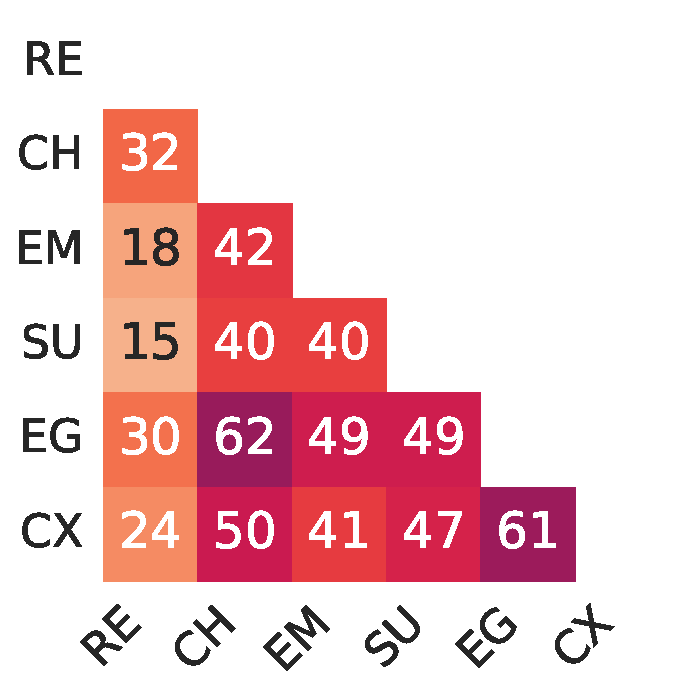
\includegraphics[width=\columnwidth]{pictures/criteria_story_kendall.pdf}
    \caption{Overall absolute Kendall correlations between human criteria. Coefficient values are multiplied by 100 for readability; we will symbolize this with ``($\times$100)'' in the next figures.}
    \label{fig:overall_human_correlations}
\end{minipage}
\hspace{0.2cm}
\begin{minipage}{0.45\columnwidth}
    \centering
    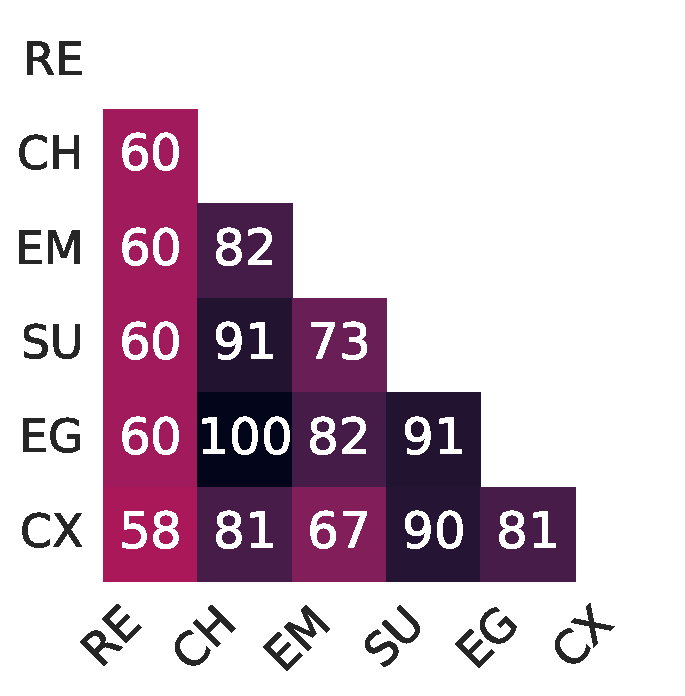
\includegraphics[width=\columnwidth]{pictures/criteria_system_kendall.pdf}
    \caption{System-level absolute Kendall correlations ($\times$100) between human criteria.}
    \label{fig:system_level_human_correlations}
\end{minipage}
\end{figure}

\paragraph{Overall Correlations (\autoref{fig:overall_human_correlations}).}
Kendall correlations range from 0.15 (\myre--\mysu) to 0.62 (\mych--\myeg), averaging at 0.40 globally. {\myeg} correlates slightly more with {\mych} and {\mycx}; this corroborates the idea that coherent and intricate plots make readers more likely to connect with a story. In contrast, {\myre} correlates on average poorly with the other criteria, which makes sense: an excellent story in every other aspect can be completely unrelated to a prompt, and vice versa. Overall, the moderate to weak correlations suggest that our criteria evaluate distinct aspects of storytelling which cannot be regrouped in fewer criteria.

\paragraph{System-level Correlations (\autoref{fig:system_level_human_correlations}).}
Compared to overall correlations, system-level correlations are higher, ranging from 0.58 (\myre--\mycx) to 1.00 (\mych--\myeg). This suggests that a given system tends to be uniformly better or worse than other systems across all criteria. Apart from this observation, the criteria tend to behave similarly. In particular, {\myre} has on average lower correlations with the other criteria.

\paragraph{Takeaways.}
The moderate to weak overall correlations between our human criteria are convincing evidence that they constitute a set of orthogonal criteria suited for human evaluation of \asg. At the system-level, we observe that current models are not specialized for a particular criterion: the high correlations suggest that a given system A tends to be uniformly better or worse than another system B across all criteria.

\subsection{Comparing {\asg} Systems}
\label{sub:comparing_asg_systems}

\begin{table}[h!]
\centering
\begin{tabular}{l@{\hskip 1em}r@{\hskip 1em}r@{\hskip 1em}r@{\hskip 1em}r@{\hskip 1em}r@{\hskip 1em}r@{\hskip 1em}r}
\toprule
Model & \multicolumn{1}{c}{{\myre}} & \multicolumn{1}{c}{{\mych}} & \multicolumn{1}{c}{{\myem}} & \multicolumn{1}{c}{{\mysu}} & \multicolumn{1}{c}{{\myeg}} & \multicolumn{1}{c}{{\mycx}} & \multicolumn{1}{c}{Average} \\
\midrule
Human          &  \result{4.17}{0.14} & \result{4.43}{0.10} &  \result{3.22}{0.14} &  \result{3.15}{0.15} &  \result{3.88}{0.12} &  \result{3.73}{0.13} & \result{3.76}{0.06} \\
\midrule
\bertgen &  \result{2.46}{0.16} &  \result{3.14}{0.16} &  \result{2.28}{0.13} &  \result{\textbf{2.09}}{0.13} &  \result{2.67}{0.12} &  \result{2.41}{0.11} & \result{2.51}{0.06} \\
\ctrl           &  \result{2.54}{0.16} &  \result{2.93}{0.16} &  \result{2.26}{0.13} &  \result{1.93}{0.12} &  \result{2.53}{0.12} &   \result{2.23}{0.10} & \result{2.40}{0.06} \\
\gpt            &   \result{2.40}{0.16} &  \result{\textbf{3.22}}{0.15} &  \result{\textbf{2.37}}{0.12} &  \result{\textbf{2.13}}{0.13} &  \result{2.76}{0.13} &  \result{2.49}{0.12} & \result{2.56}{0.06} \\
\gptt          &  \result{\textbf{\textcolor{blue}{2.81}}}{0.16} &  \result{\textbf{3.29}}{0.14} &  \result{\textbf{\textcolor{blue}{2.47}}}{0.12} & \result{\textbf{2.21}}{0.13} &  \result{\textbf{2.86}}{0.12} &   \result{2.68}{0.10} & \result{\textbf{2.72}}{0.06} \\
\gpttag    &  \result{\textbf{2.67}}{0.16} &  \result{\textbf{\textcolor{blue}{3.31}}}{0.15} &  \result{\textbf{\textcolor{blue}{2.47}}}{0.12} &  \result{\textbf{\textcolor{blue}{2.22}}}{0.13} &  \result{\textbf{\textcolor{blue}{2.92}}}{0.12} &   \result{\textbf{\textcolor{blue}{2.80}}}{0.11} & \result{\textbf{\textcolor{blue}{2.73}}}{0.06} \\
\roberta        &  \result{2.54}{0.16} &  \result{3.22}{0.16} &  \result{2.27}{0.12} &  \result{\textbf{2.12}}{0.13} &  \result{2.74}{0.12} &  \result{2.41}{0.11} & \result{2.55}{0.06} \\
\xlnet          &  \result{2.39}{0.17} &  \result{2.88}{0.16} &   \result{2.10}{0.12} &  \result{1.95}{0.12} &  \result{2.46}{0.13} &  \result{2.36}{0.11} & \result{2.36}{0.06} \\
\midrule
\fusion         &  \result{2.09}{0.16} &  \result{2.86}{0.16} &  \result{1.99}{0.12} &  \result{1.72}{0.12} &  \result{2.27}{0.14} & \result{ 1.92}{0.11} & \result{2.14}{0.06} \\
\hint           &  \result{2.29}{0.16} &  \result{2.38}{0.16} &  \result{1.74}{0.13} &  \result{1.56}{0.11} &  \result{1.75}{0.12} &   \result{1.45}{0.10} & \result{1.86}{0.06}\\
\tdvae         &  \result{2.51}{0.16} &  \result{2.99}{0.15} &  \result{2.07}{0.11} &   \result{\textbf{2.10}}{0.12} &  \result{2.59}{0.12} &  \result{2.49}{0.11} & \result{2.46}{0.06} \\
\bottomrule
\end{tabular}
\caption{Average system ratings per criterion with 95\% confidence interval. Best value in \textcolor{blue}{\textbf{bold blue}}, values in the confidence interval of the best value in \textbf{bold} without asterisk. Higher is better.}
\label{tab:system_averages}
\end{table}

\autoref{tab:system_averages} shows the average system ratings from our annotation experiment on {\hanna} V1 {\wrt}\ each of our human criteria. First, we observe that human stories achieve significantly higher scores than generated stories. Moreover, generic fine-tuned models perform better than {\asg}-specific systems, according to human annotators. The overall best system is {\gptt}, which scores better than all other systems on all criteria. The {\gptt} variant trained with {\eoptag} tags shows marginal improvement compared to {\gptt}, as reported in \citet{bai2021semantics}. It is worth noting that all models are still noticeably below human performance.

\subsection{Need for a {\hanna} Upgrade}
Soon after we released {\hanna} V1, the Natural Language Processing field underwent yet another series of advances spearheaded by the rise of Large Language Models (LLM) such as {\gptthree} \citep{brown2020language}, {\lamda} \citep{thoppilan2022lamda}, {\palm} \citep{chowdhery2022palm} and {\llama} \citep{touvron2023llama}. These new models have been setting new state-of-the-art performance standards for a wide array of {\nlp} tasks, \eg\ question answering, summarization, and machine translation. In particular, for \asg, {\llm}s are now able to produce convincing stories, so much so that they can be hard to distinguish from human stories \citep{clark2021all}. As their performance improves, they may become valuable assistants to our creative process; already, writing contests have been shown to encourage their use \citep{edilivre2023concours}.

\section{Augmenting {\hanna} with {\llmfull}s}
\label{sec:hanna_v2}

The increased availability of LLMs to the general public underlines the need for reliable story evaluation methods that can be used to improve both the performance of ASG models and our understanding of their strengths and weaknesses. Since the human annotation of stories is costly and time-consuming \citep{celikyilmaz2020evaluation}, Automatic Story Evaluation (ASE) using {\llm}s could provide an efficient and scalable replacement for human evaluation.

In this section, we use LLMs to produce new stories for {\hanna} and perform several annotation experiments where we ask LLMs to rate stories according to different human criteria and to explain their rating. We show an example of Eval-prompt and answer in \autoref{fig:demo_example}.

\begin{figure}[h!]
    \begin{framed}
    \underline{Eval-Prompt}\\
    
    \noindent \textbf{Prompt}: A mirror shows your reflection and your future soulmate. You only see your reflection.\\
    
    \noindent \textbf{Story}: Carnival music seemed to dance in the background. A cacophony of color and knick knacks decorated the fairgrounds. It was just another day at the carnival. I sit at my stand reading another old junky sci-fi novel. ``So how much to see it?'' Some pre-teen girl interrupted my book with her piercing voice. I sigh towards her and lean in. ``Ten dollars, just like the sign says.'' ``And it works?'' ``So I'm told.'' ``You mean you've never looked?'' ``Nope,'' I say, picking my book back up. ``Well why not.'' ``Because some things in this life should be a mystery,'' I reply. ``Well I want to see,'' she says. I tap on the money box and she places her ten dollars in. I watch her go in and wait for the audible reaction. After a couple of seconds I can hear an excited squeal. She runs out jumping up and down. ``He's so handsome!'' I can see her run off in excitement. I smirk. Another idiot, I think to myself. The carnival director walks up shortly after. ``Time to start packing up, Isaac,'' he says. I nod and begin to break down my stand. My table is put away, and the money is locked up now. It's that time again to put away the mirror. I stand in front of it like every other day. It's just me, again. Same as yesterday, and the day before that, I am alone in the reflection. I smile at my reflection as I cover the mirror. I put the tent and everything in the back of my trailer with a skip in my step. You have to feel sorry for these suckers, I think. They're destined for one person only. Who knows if they'll ever find them? At least I know where to always find myself.\\
    
    Rate the story on a scale from 1 to 5 on Empathy and explain your answer.\\
    
    Rating:
    \end{framed}
    \begin{framed}
    \underline{LLM Answer}\\
    
    I would rate the story a 2 on Empathy. While I could relate to the character's feelings of indifference towards the magic mirror, I did not feel a strong emotional connection to any of the characters. There were no specific emotions that I recognized in the characters, and I could not completely relate to them on an emotional level.
    \end{framed}
    \caption{Example Eval-Prompt and answer from our experiments. ``Prompt'' inside the Eval-Prompt refers to the story-prompt.}
    \label{fig:demo_example}
\end{figure}

We release this second version of {\hanna}, which we will call {\hanna} V2, on GitHub\footnote{\url{https://github.com/dig-team/hanna-benchmark-asg}}. Our data consists of:
\begin{itemize}
    \item \textbf{ASG experiment}: 480 stories generated by Llama models with corresponding LLM annotations to expand the \hanna\ corpus;
    \item \textbf{ASE experiments}: $\sim$150k rating and explanation annotations (1,056 stories, 6 criteria, 4 Eval-Prompts, 3 tries, 2 models).
\end{itemize}

\subsection{Experimental Protocol for {\asg} using {\llm}s}
\label{sub:llm_methodology_asg}

\begin{table}[h!]
\small
\centering
\begin{tabular}{p{0.3\columnwidth}p{0.3\columnwidth}p{0.3\columnwidth}}
\toprule
    \multicolumn{3}{c}{\textbf{Prompt}} \\
    \multicolumn{3}{p{0.9\columnwidth}}{Write a story about an elderly wizard and his young female apprentice.} \\
\midrule
    \multicolumn{1}{c}{\textbf{Llama-7B Story}} & \multicolumn{1}{c}{\textbf{{\beluga} Story}} & \multicolumn{1}{c}{\textbf{{\platypus} Story}} \\
    It was a crisp autumn day when the elderly wizard, Orion, welcomed his new apprentice, Lily, to his tower. Orion had been searching for a worthy successor for many years, and he had finally found the perfect person in Lily. She was a bright and curious young woman, eager to learn the ways of magic. As Lily entered the tower, she was struck by its grandeur. It was filled with ancient tomes, dusty artifacts, and mysterious creatures. [\dots] & In the enchanted realm of Cascadia, a wise old wizard named Elder Oak lived in solitude, guarding the ancient forest's secrets and magic. The trees seemed to whisper, and the winds sighed their stories to him, for he was the last of his kind. He spent his days learning and protecting the natural wisdom, and his nights were filled with dreams of a future where the wonders of his world were cherished and honored. [\dots] & Once upon a time, in the faraway magical kingdom of Alvoria, there lived an elderly wizard named Azmandor. Azmandor had dedicated his entire life to the pursuit of knowledge, particularly in the field of magic. His quest had brought him great fame and recognition among his peers, but little happiness. Now, as he approached the twilight of his life, he longed for a new apprentice to pass on his vast store of magical knowledge. [\dots] \\
\bottomrule
\end{tabular}
\caption{Example aligned stories from Llama-7B, \beluga, and \platypus.}
\label{tab:asg_llm_stories}
\end{table}

Since the release of the {\hanna} V1 dataset, language models have made significant advancements. We therefore feel the need to expand {\hanna} with stories generated by more recent models and, namely, Large Language Models ({\llm}s). We consider the source-available Llama2 models \citep{touvron2023llama2} for that purpose.

We select \texttt{Llama-2-7b-chat-hf} (Llama-7B) as a new baseline and 4 high-performing models (at the time of selection) of different sizes on the HuggingFace Open LLM Leaderboard\footnote{\url{https://huggingface.co/spaces/HuggingFaceH4/open_llm_leaderboard}}: 

\begin{enumerate}[noitemsep]
    \item \texttt{Platypus2-70B-instruct} (\platypus),
    \item \texttt{llama-30b-instruct-2048} (\llamalarge),
    \item \texttt{StableBeluga-13B} (\beluga),
    \item \texttt{Mistral-7B-OpenOrca} (\mistral).
\end{enumerate}

We use the following LLM-prompt, where ``PROMPT'' is replaced by a given story-prompt:

\begin{verbatim}
    ### Human: Write a story based off the prompt given below.
    
    Prompt: {PROMPT}
    
    ### Assistant:
\end{verbatim}

As a result, we obtain 480 new stories generated with 5 {\llmfull}s. See \autoref{tab:asg_llm_stories} for an example of aligned stories. We can observe that, compared with older {\asg}-specific models (\autoref{tab:asg_model_stories}), the stories generated by {\llm}s appear to be much more fluent. 

\subsection{Experimental Protocol for Automatic Annotation using LLMs}
\label{sub:llm_methodology_ase}

In this section, we use LLMs as {\asefull} measures. We will refer to the prompt that is fed to the LLM as the \textit{Eval-Prompt}, to distinguish it from the story-prompt. See \autoref{fig:demo_example} for an example of the use of an LLM for story evaluation and \autoref{fig:llm_schema} for a schematic overview of our experiments.

\subsubsection{Related work}
\label{ssub:llm_related_work}

\paragraph{Automatic Annotation with LLMs.}
LLMs are increasingly being tested for automatic text annotation, \textit{e.g.}\ for sentiment analysis  \citep{qureshi2022novel}, named entity recognition \citep{enkhsaikhan2021auto} or event structure modeling \citep{vauth2021automated}.
\citet{wang2021want} propose to leverage {\gptthree} as a data labeler and show that it can be up to 96\% more cost-efficient than human labeling on a variety of NLP tasks. They also explore various strategies of mixing labeled data from {\gptthree} and humans under a fixed budget and achieve better performance than using data from a single labeler.
\citet{ding2022gpt} conduct a comprehensive analysis on using {\gptthree} for data annotation for complex NLP tasks. They find that directly annotating unlabeled data is suitable for tasks with small label space (\eg\ binary stance classification) while generation-based methods are more suitable for tasks with large label space (\eg\ neural entity recognition). Overall, they find that generation-based approaches tend to be more cost-effective compared with human annotation of unlabeled data, but that {\gptthree} annotations are still of inferior quality compared with human annotations.
\citet{chakrabarty2023art} design the Torrance Test for Creative Writing (TTCW), a set of 14 tests based on the four original Torrance dimensions of fluency, flexibility, originality, and elaboration. They experimentally validate the TTCW through an assessment of 48 stories written by humans or generated by LLMs and involving 10 participants with expertise in creative writing. They find that the experts reach moderate agreement on individual dimensions, and strong agreement when evaluating all dimensions in aggregate. They show that LLM-generated stories are three to ten times less likely to pass TTCW tests compared to expert-written stories, and that current state-of-the-art LLMs are not yet capable of reproducing expert assessments when administering TTCW tests. We seek to generalize their findings through a larger-scale evaluation (1,000+ stories), a more diverse pool of LLMs, including source-available models, and a finer analysis and discussion of LLM performance.

\paragraph{Prompt Engineering.}
The importance of designing efficient prompts for large language models such as {\gptthree} has been extensively investigated in recent years. A systematic survey of prompt engineering techniques can be found in \citet{sahoo2024systematic}: they explain that zero-shot and few-shot prompting were the first paradigms that emerged with LLMs. Those setups were generally sufficient, except for more reasoning-oriented tasks, to which LLMs failed more often. Chain-of-Thought prompting \citep{wei2022chain} was therefore developed, soon followed by multiple variants.
\citet{radford2019language} use zero-shot prompting for benchmarking their {\gptt} model. This technique removes the need for extensive training data, instead relying on carefully crafted prompts that guide the model toward novel tasks. They find that GPT-2 zero-shots to state-of-the-art performance on 7 out of 8 tested language modeling datasets, and they surmise that high-capacity models trained to maximize the likelihood of a sufficiently varied text corpus become unsupervised multitask learners. \citet{brown2020language} introduce the {\gptthree} language model and test its performance in a few-shot setting, where the model is given a few input-output examples to help it grasp the task at hand. They demonstrate that, in contrast to zero-shot prompting, a few high-quality examples are enough to enhance model performance on complex tasks. However, few-shot prompting could be less adapted to longer text inputs, as it needs extra tokens for the examples. Furthermore, they discover that biases like favoring frequent terms may have an impact on few-shot results, and that the design of the provided examples greatly influence model behavior. \citet{reynolds2021prompt} notably find that zero-shot prompting can perform similarly to few-shot prompting, and even exceed it. They explore the design of metaprompts that prime the language model to better solve a given problem. \citet{zhou2022large} treat the prompt engineering process as an optimization problem, use search algorithms guided by LLMs to solve it and attain human-level performance.
\citet{wei2022chain} introduce Chain-of-Thought (CoT), a prompting strategy that enables models to decompose complex problems into simpler steps. Through a series of experiments, they demonstrate that CoT prompting improve model performance for both commonsense and symbolic reasoning. They achieve state-of-the-art results in math and commonsense reasoning benchmarks with {\palm} 540B, reaching an accuracy of 90.2\%. \citet{wei2022emergent} and \citet{white2023prompt} review different strategies that have been applied to augment large language model abilities, \textit{e.g.}\ least-to-most prompting \citep{zhou2022least}, ask-me-anything prompting \citep{arora2022askma}, and zero-shot chain-of-thought reasoning \citep{kojima2022large}.\\

In our setting, we choose to investigate whether LLMs perform better with simple or detailed guidelines, and with zero- or one-shot Eval-Prompts.


\begin{figure}[!h]
    \centering
    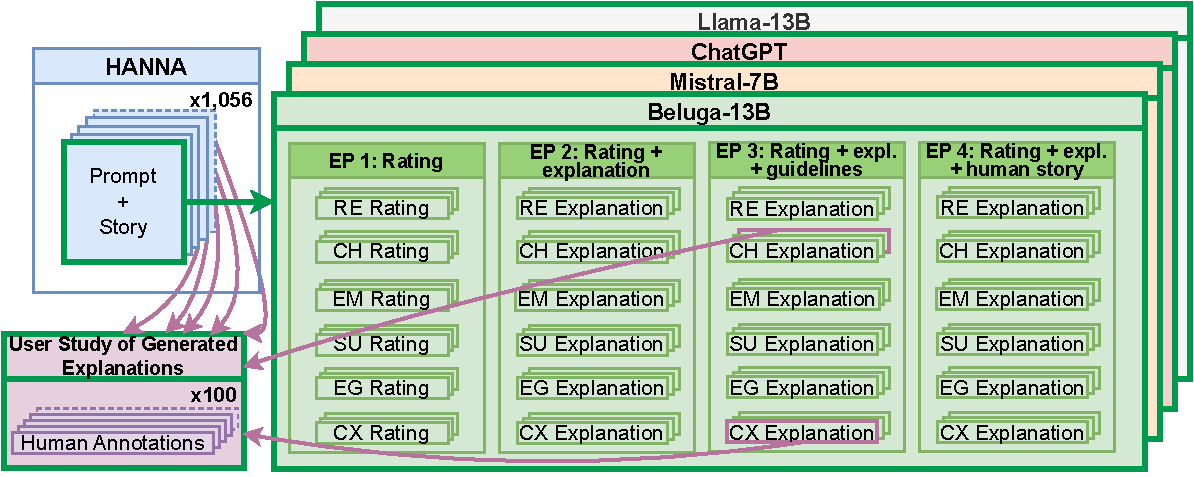
\includegraphics[width=\columnwidth]{pictures/llm_schema.pdf}
    \caption{Schema of the performed ASE experiments. RE, CH, etc. are the considered human criteria. ``EP'' means ``Eval-Prompt'', defined in \autoref{sub:llm_methodology_ase}. For the user study (\autoref{sub:llm_user_study}), we randomly sampled 100 explanations from our experiments.}
    \label{fig:llm_schema}
\end{figure}

\subsubsection{ASE Criteria} We re-use our set of six human criteria introduced in \autoref{sub:our_criteria}:
\begin{enumerate}[noitemsep]
    \item \textbf{Relevance} ({\myre}, how well the story matches its prompt), 
    \item \textbf{Coherence} ({\mych}, how much the story makes sense), 
    \item \textbf{Empathy} ({\myem}, how well the reader understood the character's emotions),
    \item \textbf{Surprise} ({\mysu}, how surprising the end of the story was),
    \item \textbf{Engagement} ({\myeg}, how much the reader engaged with the story),
    \item \textbf{Complexity} ({\mycx}, how elaborate the story is).
\end{enumerate}

\subsubsection{Methodology}
Given the importance of good prompt engineering \citep{zhao2021calibrate}, we design four different Eval-Prompts for the generation of ratings. For each of our Eval-Prompts, we provide the model with a story-prompt and a corresponding story. Then:

\begin{enumerate}
    \item \textbf{Eval-Prompt 1} (simple rating): we ask the model to rate the story on a scale from 1 to 5 on one of the six criteria;
    \item \textbf{Eval-Prompt 2} (rating with explanation): same as Eval-Prompt 1, and we ask the model to explain its answer;
    \item \textbf{Eval-Prompt 3} (rating with explanation and guidelines): same as Eval-Prompt 2, and we provide the model with the detailed guidelines from our original human annotation protocol (see \autoref{sub:hanna_v1});
    \item \textbf{Eval-Prompt 4} (rating with explanation and human story): same as Eval-Prompt 2, and we provide the model with the human story associated with the same story-prompt. We explicitly tell the model that the human story is only given for reference purposes.
\end{enumerate}

Different Eval-Prompt examples can be found in Figures \ref{fig:eval_prompt_1}, \ref{fig:eval_prompt_2}, \ref{fig:eval_prompt_3}, and \ref{fig:eval_prompt_4}.

\begin{figure}[h!]
    \begin{framed}
    \underline{Eval-Prompt 1}\\
    
    \noindent \textbf{Prompt}: You have become death, destroyer of worlds.\\
    
    \noindent \textbf{Story}: You look up to see all of them in fear. You just must fix this soon. Slowly, just like your Father always had instructed him, you look down and see all your foes dead and beaten down. You can't resist the urge to touch the wounds. For there is nothing you can do about it. [...]\\
    
    Rate the story on a scale from 1 to 5 on Surprise (how surprising the end of the story was).\\
    
    Rating:
    \end{framed}
    \caption{Example of an Eval-Prompt 1 for the Surprise criterion.}
    \label{fig:eval_prompt_1}
\end{figure}

\begin{figure}[h!]
    \begin{framed}
    \underline{Eval-Prompt 2}\\
    
    \noindent \textbf{Prompt}: You have become death, destroyer of worlds.\\
    
    \noindent \textbf{Story}: You look up to see all of them in fear. You just must fix this soon. Slowly, just like your Father always had instructed him, you look down and see all your foes dead and beaten down. You can't resist the urge to touch the wounds. For there is nothing you can do about it. [...]\\
    
    Rate the story on a scale from 1 to 5 on Surprise (how surprising the end of the story was) and explain your answer.\\
    
    Rating:
    \end{framed}
    \caption{Example of an Eval-Prompt 2 for the Surprise criterion.}
    \label{fig:eval_prompt_2}
\end{figure}

\begin{figure}[h!]
    \begin{framed}
    \underline{Eval-Prompt 3}\\
    
    \noindent \textbf{Prompt}: You have become death, destroyer of worlds.\\
    
    \noindent \textbf{Story}: You look up to see all of them in fear. You just must fix this soon. Slowly, just like your Father always had instructed him, you look down and see all your foes dead and beaten down. You can't resist the urge to touch the wounds. For there is nothing you can do about it. [...]\\
    
    \noindent \textbf{Guidelines}:\\
    1 — The ending seemed completely obvious from the start, or doesn't make any sense at all.\\
    2 — The ending was easily predictable after a few sentences.\\
    3 — The ending was predictable after half of the story.\\
    4 — The ending surprised you, but would have been difficult to predict.\\
    5 — The ending surprised you, and still seemed as if it could very reasonably have been predicted, ie, there were enough clues in the story.\\
    
    Rate the story on a scale from 1 to 5 on Surprise (how surprising the end of the story was) and explain your answer. Use the provided guidelines.\\
    
    Rating:
    \end{framed}
    \caption{Example of an Eval-Prompt 3 for the Surprise criterion.}
    \label{fig:eval_prompt_3}
\end{figure}

\begin{figure}[h!]
    \begin{framed}
    \underline{Eval-Prompt 4}\\
    
    \noindent \textbf{Prompt}: You have become death, destroyer of worlds.\\
    
    \noindent \textbf{Target Story}: You look up to see all of them in fear. You just must fix this soon. Slowly, just like your Father always had instructed him, you look down and see all your foes dead and beaten down. You can't resist the urge to touch the wounds. For there is nothing you can do about it. [...]\\
    
    \noindent \textbf{Human Story}: I saw the button. It was simple, red, no words on it as I already knew what it did. I mean I built the button, I built what happens when you press the button, and I was given the choice of whether or not to push the button. Humanity was screwed, that much was apparent, Plagues and starvation across 3 planets and 6 space stations. [...]\\
    
    Rate the target story on a scale from 1 to 5 on Surprise (how surprising the end of the story was) and explain your answer. Do not rate the human story; it is here only for reference.\\
    
    Rating:
    \end{framed}
    \caption{Example of an Eval-Prompt 4 for the Surprise criterion.}
    \label{fig:eval_prompt_4}
\end{figure}

\clearpage

\subsubsection{{\asefull} Models}

We consider source-available Llama-2 \citep{touvron2023llama2} models for our experiments, and the closed-source \texttt{gpt-3.5-turbo} model from OpenAI. Precisely, we use the 5 following models: 

\begin{enumerate}[noitemsep]
    \item \texttt{StableBeluga-13B} (Beluga-13B),
    \item \texttt{Llama-2-13b-chat-hf} (Llama-13B),
    \item \texttt{Mistral-7B-OpenOrca} (Mistral-7B),
    \item \texttt{Llama-2-7b-chat-hf} (Llama-7B),
    \item \texttt{gpt-3.5-turbo} (ChatGPT).
\end{enumerate}

Llama-2 models were trained on a closed ``new mix of data from publicly available sources''. Beluga-13B and Mistral-7B are Llama-2 models fine-tuned on Orca-style datasets which contain triplets of ``System message--User query--LLM response'' for a large collection of tasks \citep{mukherjee2023orca}. Beluga-13B is fine-tuned on StabilityAI's closed internal dataset, while Mistral-7B is fine-tuned on the open OpenOrca dataset \citep{lian2023openorca}. 

ChatGPT \citep{brown2020language, ouyang2022training} is a closed-source model trained on a closed internal dataset that includes the CommonCrawl, Books1 and Books2 datasets.

We submit each of the four Eval-Prompts 3 times on all 1,056 {\hanna} stories on each of the 6 criteria, and we then extract the ratings automatically from the generated answer via a regular expression. Since story evaluation on multiple prompts and multiple criteria is computationally demanding, we limit our experiments to 13B and 7B models.

{\llamasmall} failed at the task too often for the results to be exploitable, \textit{e.g.}\ by generating nonsensical conversations between itself and the user: in more than half of its answers, no rating was provided at all, so we excluded it from our analysis.

We use the default parameter values, \ie, $(\textrm{temperature}, \textrm{top\_p}) = (1, 0.95)$ for Llama models and $(0.7, 1)$ for ChatGPT.

\subsubsection{Libraries} We use the {\transf} library \citep{wolf-etal-2020-transformers} and the OpenAI API for our experiments.

\begin{table}[!h]
\small
\centering
\begin{tabular}{lccccccc}
\toprule
\textbf{Model} & \textbf{RE} & \textbf{CH} & \textbf{EM} & \textbf{SU} & \textbf{EG} & \textbf{CX} & \textbf{Average} \\
\midrule
Human             &  \result{3.37}{0.12} &  \result{3.55}{0.11} &  \result{3.42}{0.11} &  \result{3.11}{0.13} &  \result{3.58}{0.10} &  \result{3.48}{0.10} &  \result{3.42}{0.06} \\
\midrule
Platypus2-70B     &  \result{4.09}{0.05} &  \result{4.31}{0.05} &  \result{3.92}{0.06} &  \result{\textbf{\textcolor{blue}{3.69}}}{0.07} &  \result{4.19}{0.05} &  \result{3.88}{0.05} &  \result{4.01}{0.03} \\
Llama-30B & \result{\textbf{\textcolor{blue}{4.19}}}{0.05} &  \result{\textbf{\textcolor{blue}{4.38}}}{0.04} &  \result{\textbf{\textcolor{blue}{4.04}}}{0.06} &  \result{\textbf{3.63}}{0.09} &  \result{\textbf{\textcolor{blue}{4.31}}}{0.05} &  \result{\textcolor{blue}{\textbf{3.98}}}{0.05} &  \result{\textbf{\textcolor{blue}{4.08}}}{0.03} \\
Beluga-13B        &  \result{4.06}{0.08} &  \result{4.10}{0.06} &  \result{3.75}{0.08} &  \result{3.54}{0.08} &  \result{3.90}{0.08} &  \result{3.69}{0.07} &  \result{3.84}{0.05} \\
Mistral-7B    &  \result{4.12}{0.05} &  \result{4.25}{0.05} &  \result{3.86}{0.06} &  \result{3.56}{0.08} &  \result{4.11}{0.05} &  \result{3.82}{0.04} &  \result{3.95}{0.03} \\
Llama-7B      &  \result{4.07}{0.06} &  \result{4.24}{0.05} &  \result{3.90}{0.06} &  \result{3.58}{0.06} &  \result{4.09}{0.05} &  \result{3.79}{0.05} &  \result{3.95}{0.03} \\
GPT-2             &  \result{2.57}{0.13} &  \result{2.36}{0.11} &  \result{2.72}{0.11} &  \result{2.59}{0.14} &  \result{2.67}{0.12} &  \result{2.89}{0.12} &  \result{2.63}{0.07} \\
HINT              &  \result{1.57}{0.10} &  \result{1.31}{0.07} &  \result{1.59}{0.10} &  \result{1.49}{0.10} &  \result{1.58}{0.09} &  \result{1.43}{0.08} &  \result{1.49}{0.06} \\
\bottomrule
\end{tabular}
\caption{Average Beluga-13B ratings for Eval-Prompt 1 with 95\% confidence interval. Higher is better.}
\label{tab:average_beluga_ratings}
\end{table}

\begin{table}[!h]
\small
\centering
\begin{tabular}{lccccccc}
\toprule
\textbf{Model} & \textbf{RE} & \textbf{CH} & \textbf{EM} & \textbf{SU} & \textbf{EG} & \textbf{CX} & \textbf{Average} \\
\midrule
Human             &  \result{3.48}{0.11} &  \result{3.50}{0.10} &  \result{3.69}{0.08} &  \result{3.24}{0.11} &  \result{3.42}{0.10} &  \result{3.45}{0.07} &  \result{3.46}{0.05} \\
\midrule
Platypus2-70B     &  \result{\textbf{\textcolor{blue}{4.26}}}{0.08} &  \result{\textbf{\textcolor{blue}{4.31}}}{0.08} &  \result{\textbf{\textcolor{blue}{4.05}}}{0.07} &  \result{\textbf{3.46}}{0.10} &  \result{\textbf{\textcolor{blue}{3.94}}}{0.06} &  \result{3.55}{0.07} &  \result{\textbf{\textcolor{blue}{3.93}}}{0.03} \\
Llama-30B &  \result{4.15}{0.10} &  \result{\textbf{4.29}}{0.07} &  \result{\textbf{4.02}}{0.07} &  \result{\textbf{3.46}}{0.09} &  \result{\textbf{\textcolor{blue}{3.94}}}{0.06} &  \result{\textbf{3.65}}{0.07} &  \result{\textbf{3.92}}{0.03} \\
Beluga-13B        &  \result{4.07}{0.09} &  \result{4.14}{0.07} &  \result{3.98}{0.07} &  \result{\textbf{3.50}}{0.09} &  \result{3.74}{0.08} &  \result{3.59}{0.07} &  \result{3.84}{0.03} \\
Mistral-7B    &  \result{4.15}{0.10} &  \result{4.22}{0.08} &  \result{\textbf{4.02}}{0.07} &  \result{\textbf{\textcolor{blue}{3.51}}}{0.11} &  \result{\textbf{\textcolor{blue}{3.94}}}{0.07} &  \result{\textbf{\textcolor{blue}{3.67}}}{0.07} &  \result{\textbf{3.92}}{0.04} \\
Llama-7B      &  \result{4.13}{0.10} &  \result{4.14}{0.09} &  \result{3.90}{0.08} &  \result{\textbf{3.48}}{0.09} &  \result{3.78}{0.08} &  \result{3.56}{0.08} &  \result{3.83}{0.05} \\
GPT-2             &  \result{2.40}{0.10} &  \result{2.37}{0.09} &  \result{2.74}{0.10} &  \result{2.85}{0.11} &  \result{2.60}{0.09} &  \result{2.88}{0.09} &  \result{2.64}{0.05} \\
HINT              &  \result{2.12}{0.11} &  \result{2.13}{0.08} &  \result{2.23}{0.10} &  \result{2.28}{0.11} &  \result{2.05}{0.08} &  \result{2.05}{0.09} &  \result{2.15}{0.06} \\
\bottomrule
\end{tabular}
\caption{Average Mistral-7B ratings for Eval-Prompt 1 with 95\% confidence interval. Higher is better.}
\label{tab:average_mistral_ratings}
\end{table} 

\subsection{LLM Performance at {\asg}}
\label{sub:asg1_analysis}

In \autoref{tab:average_beluga_ratings} and \autoref{tab:average_mistral_ratings}, we display the average ratings attributed by respectively {\beluga} and {\mistral} to multiple V1 and V2 systems. For the sake of readability, we restrict the scope of the tables to human stories, {\llm} stories and {\gptt} and {\hint}, respectively the best and worst systems from {\hanna} V1. Other V1 systems have similar ratings to the latter two.

We observe that, according to {\beluga} and {\mistral}, LLMs perform remarkably well, getting higher ratings than older models (GPT-2) and even human stories. Beluga-13B and Mistral-7B both seem to prefer the outputs from larger LLMs (Platypus2-70B, Llama-30B) to their own outputs, suggesting that the LLM grading process cannot be explained simply by a proxy for perplexity. Interestingly, in both tables, Mistral-7B gets slightly higher ratings than Beluga, with some differences being statistically discernible, which could be explained by differences in fine-tuning data.

\paragraph{Takeaways.} Larger models (Platypus2-70B, Llama-30B) exhibit the best ASG performance, with LLM ratings at least equal to those of human stories. However, our setting involves short stories of between 500 and 1,000 words; generating longer stories may prove more difficult since maintaining large-scale coherence may become an issue. Moreover, we need to confirm that {\asefull} performed by {\llm}s is reliable proxy for human evaluation: we tackle this question in \autoref{sec:llms_for_ase}.

\section{Conclusion}

Motivated by our survey of the \asgfull\ literature (\autoref{sec:decision_process_hanna}), we built \hanna, a new corpus designed for {\asg} evaluation. The first version of {\hanna} contains 1,056 stories written or generated by 11 systems (1 human writer, 3 ASG-specific systems, and 7 pretrained language models), and aligned on 96 prompts (\autoref{sub:hanna_v1}) We performed an annotation experiment on {\hanna} V1, asking human raters to grade each story {\wrt}\ our six human criteria. We computed intra-class coefficients to estimate the consistency of our 19,0008 annotations and found that our values are in tune with the existing NLP literature (\autoref{sub:inter_rater_reliability_hanna}).

Furthermore, we analyzed the overall and system-level correlations between our human criteria, and confirmed that they allow for a standardized and extensive human evaluation (\autoref{sub:evaluating_human_criteria}). Indeed, our six criteria are moderately to weakly correlated with one another, which shows that they are non-redundant, and produce coherent system rankings. Additionally, we observed that large pre-trained language models produce the best results for ASG (\autoref{sub:comparing_asg_systems}). In particular, \gptt\ performed better than systems specifically tailored for ASG despite being older than some of them. Overall, all systems remained significantly inferior to human output.

Finally, we used {\llmfull}s to augment {\hanna} with 480 new stories (\autoref{sub:llm_methodology_asg}) and 150k+ annotations containing ratings of stories {\wrt}\ different Eval-Prompts and human criteria (\autoref{sub:llm_methodology_ase}). We also observed that {\llm}s obtain better grades than humans when evaluated by two different {\llm}s: {\beluga} and {\mistral} (\autoref{sub:asg1_analysis}).

In \autoref{chap:meta_evaluation}, we conduct our meta-evaluation benchmark of automatic measures on \hanna\, and evaluate the performance of {\llmfull}s on {\asefull}.